% Options for packages loaded elsewhere
\PassOptionsToPackage{unicode}{hyperref}
\PassOptionsToPackage{hyphens}{url}
%
\documentclass[
]{book}
\usepackage{amsmath,amssymb}
\usepackage{lmodern}
\usepackage{ifxetex,ifluatex}
\ifnum 0\ifxetex 1\fi\ifluatex 1\fi=0 % if pdftex
  \usepackage[T1]{fontenc}
  \usepackage[utf8]{inputenc}
  \usepackage{textcomp} % provide euro and other symbols
\else % if luatex or xetex
  \usepackage{unicode-math}
  \defaultfontfeatures{Scale=MatchLowercase}
  \defaultfontfeatures[\rmfamily]{Ligatures=TeX,Scale=1}
\fi
% Use upquote if available, for straight quotes in verbatim environments
\IfFileExists{upquote.sty}{\usepackage{upquote}}{}
\IfFileExists{microtype.sty}{% use microtype if available
  \usepackage[]{microtype}
  \UseMicrotypeSet[protrusion]{basicmath} % disable protrusion for tt fonts
}{}
\makeatletter
\@ifundefined{KOMAClassName}{% if non-KOMA class
  \IfFileExists{parskip.sty}{%
    \usepackage{parskip}
  }{% else
    \setlength{\parindent}{0pt}
    \setlength{\parskip}{6pt plus 2pt minus 1pt}}
}{% if KOMA class
  \KOMAoptions{parskip=half}}
\makeatother
\usepackage{xcolor}
\IfFileExists{xurl.sty}{\usepackage{xurl}}{} % add URL line breaks if available
\IfFileExists{bookmark.sty}{\usepackage{bookmark}}{\usepackage{hyperref}}
\hypersetup{
  pdftitle={Simulation and Modelling to Understand Change},
  pdfauthor={Manuele Leonelli},
  hidelinks,
  pdfcreator={LaTeX via pandoc}}
\urlstyle{same} % disable monospaced font for URLs
\usepackage{color}
\usepackage{fancyvrb}
\newcommand{\VerbBar}{|}
\newcommand{\VERB}{\Verb[commandchars=\\\{\}]}
\DefineVerbatimEnvironment{Highlighting}{Verbatim}{commandchars=\\\{\}}
% Add ',fontsize=\small' for more characters per line
\usepackage{framed}
\definecolor{shadecolor}{RGB}{248,248,248}
\newenvironment{Shaded}{\begin{snugshade}}{\end{snugshade}}
\newcommand{\AlertTok}[1]{\textcolor[rgb]{0.94,0.16,0.16}{#1}}
\newcommand{\AnnotationTok}[1]{\textcolor[rgb]{0.56,0.35,0.01}{\textbf{\textit{#1}}}}
\newcommand{\AttributeTok}[1]{\textcolor[rgb]{0.77,0.63,0.00}{#1}}
\newcommand{\BaseNTok}[1]{\textcolor[rgb]{0.00,0.00,0.81}{#1}}
\newcommand{\BuiltInTok}[1]{#1}
\newcommand{\CharTok}[1]{\textcolor[rgb]{0.31,0.60,0.02}{#1}}
\newcommand{\CommentTok}[1]{\textcolor[rgb]{0.56,0.35,0.01}{\textit{#1}}}
\newcommand{\CommentVarTok}[1]{\textcolor[rgb]{0.56,0.35,0.01}{\textbf{\textit{#1}}}}
\newcommand{\ConstantTok}[1]{\textcolor[rgb]{0.00,0.00,0.00}{#1}}
\newcommand{\ControlFlowTok}[1]{\textcolor[rgb]{0.13,0.29,0.53}{\textbf{#1}}}
\newcommand{\DataTypeTok}[1]{\textcolor[rgb]{0.13,0.29,0.53}{#1}}
\newcommand{\DecValTok}[1]{\textcolor[rgb]{0.00,0.00,0.81}{#1}}
\newcommand{\DocumentationTok}[1]{\textcolor[rgb]{0.56,0.35,0.01}{\textbf{\textit{#1}}}}
\newcommand{\ErrorTok}[1]{\textcolor[rgb]{0.64,0.00,0.00}{\textbf{#1}}}
\newcommand{\ExtensionTok}[1]{#1}
\newcommand{\FloatTok}[1]{\textcolor[rgb]{0.00,0.00,0.81}{#1}}
\newcommand{\FunctionTok}[1]{\textcolor[rgb]{0.00,0.00,0.00}{#1}}
\newcommand{\ImportTok}[1]{#1}
\newcommand{\InformationTok}[1]{\textcolor[rgb]{0.56,0.35,0.01}{\textbf{\textit{#1}}}}
\newcommand{\KeywordTok}[1]{\textcolor[rgb]{0.13,0.29,0.53}{\textbf{#1}}}
\newcommand{\NormalTok}[1]{#1}
\newcommand{\OperatorTok}[1]{\textcolor[rgb]{0.81,0.36,0.00}{\textbf{#1}}}
\newcommand{\OtherTok}[1]{\textcolor[rgb]{0.56,0.35,0.01}{#1}}
\newcommand{\PreprocessorTok}[1]{\textcolor[rgb]{0.56,0.35,0.01}{\textit{#1}}}
\newcommand{\RegionMarkerTok}[1]{#1}
\newcommand{\SpecialCharTok}[1]{\textcolor[rgb]{0.00,0.00,0.00}{#1}}
\newcommand{\SpecialStringTok}[1]{\textcolor[rgb]{0.31,0.60,0.02}{#1}}
\newcommand{\StringTok}[1]{\textcolor[rgb]{0.31,0.60,0.02}{#1}}
\newcommand{\VariableTok}[1]{\textcolor[rgb]{0.00,0.00,0.00}{#1}}
\newcommand{\VerbatimStringTok}[1]{\textcolor[rgb]{0.31,0.60,0.02}{#1}}
\newcommand{\WarningTok}[1]{\textcolor[rgb]{0.56,0.35,0.01}{\textbf{\textit{#1}}}}
\usepackage{longtable,booktabs,array}
\usepackage{calc} % for calculating minipage widths
% Correct order of tables after \paragraph or \subparagraph
\usepackage{etoolbox}
\makeatletter
\patchcmd\longtable{\par}{\if@noskipsec\mbox{}\fi\par}{}{}
\makeatother
% Allow footnotes in longtable head/foot
\IfFileExists{footnotehyper.sty}{\usepackage{footnotehyper}}{\usepackage{footnote}}
\makesavenoteenv{longtable}
\usepackage{graphicx}
\makeatletter
\def\maxwidth{\ifdim\Gin@nat@width>\linewidth\linewidth\else\Gin@nat@width\fi}
\def\maxheight{\ifdim\Gin@nat@height>\textheight\textheight\else\Gin@nat@height\fi}
\makeatother
% Scale images if necessary, so that they will not overflow the page
% margins by default, and it is still possible to overwrite the defaults
% using explicit options in \includegraphics[width, height, ...]{}
\setkeys{Gin}{width=\maxwidth,height=\maxheight,keepaspectratio}
% Set default figure placement to htbp
\makeatletter
\def\fps@figure{htbp}
\makeatother
\setlength{\emergencystretch}{3em} % prevent overfull lines
\providecommand{\tightlist}{%
  \setlength{\itemsep}{0pt}\setlength{\parskip}{0pt}}
\setcounter{secnumdepth}{5}
\usepackage{booktabs}
\ifluatex
  \usepackage{selnolig}  % disable illegal ligatures
\fi
\usepackage[]{natbib}
\bibliographystyle{apalike}

\title{Simulation and Modelling to Understand Change}
\author{Manuele Leonelli}
\date{2021-01-18}

\begin{document}
\maketitle

{
\setcounter{tocdepth}{1}
\tableofcontents
}
\hypertarget{preface}{%
\chapter*{Preface}\label{preface}}
\addcontentsline{toc}{chapter}{Preface}

These are lecture notes for the module \emph{Simulation and Modelling to Understand Change} given in the School of Human Sciences and Technology at IE University, Madrid, Spain. The module is given in the 2nd semester of the 1st year of the bachelor in Data \& Business Analytics. Knowledge of basic elements of R programming as well as probability and statistics is assumed.

\hypertarget{intro}{%
\chapter{Introduction}\label{intro}}

The first introductory chapter gives an overview of simulation, what it is, what it can be used for, as well as some examples.

\hypertarget{what-is-simulation}{%
\section{What is simulation}\label{what-is-simulation}}

A \emph{simulation} is an imitation of the dynamics of a real-world process or system over time. Although simulation could potentially still be done ``by hand'', nowadays it almost always implicitly requires the use of a computer to create an artificial history of a system to draw inferences about its characteristics and workings.

The behavior of the system is studied by constructing a \emph{simulation model}, which usually takes the form of a set of assumptions about the workings of the system. Once developed, a simulation model can be used for a variety of tasks, including:

\begin{itemize}
\item
  Investigate the behaviour of the system under a wide array of scenarios. This is also often referred to as ``what-if'' analyses;
\item
  Changes to the system can be simulated before implementation to predict their impact in real-world;
\item
  During the design stage of a system, meaning while it is being built, simulation can be used to guide its construction.
\end{itemize}

Computer simulation has been used in a variety of domains, including manifacturing, health care, transport system, defense and management science, among many others.

\hypertarget{a-simple-simulation-model}{%
\subsection{A simple simulation model}\label{a-simple-simulation-model}}

Suppose we decided to open a donut shop and are unsure about how many employees to hire to sell donuts to costumers. The operations of our little shop is the real-world system whose behavior we want to understand. Given that the shop is not operating yet, only a simulation model can provide us with insights.

We could of course devise models of different complexities, but for now suppose that we are happy with a simple model where we have the following elements:

\begin{itemize}
\item
  costumers that arrive at our shop at a particular rate;
\item
  employees (of a number to be given as input) that take a specific time to serve costumers.
\end{itemize}

Implicitly, we are completely disregarding the number of donuts available in our shop and assuming that we have an infinite availability of these. Of course, in a more complex simulation model we may want to also include this element to give a more realistic description of the system.

\hypertarget{why-simulate}{%
\subsection{Why simulate?}\label{why-simulate}}

An alternative approach to computer simulation is direct experimentation. In the bagel shop setting, we could wait for the shop to open and observe its workings by having a different number of employees on different days. Considered against real experimentation, simulation has the following advantages:

\begin{itemize}
\item
  It is \emph{cheaper} to implement and does not require a disruption of the real-world system;
\item
  It is \emph{faster} to implement and time can be compressed or expanded to allow for a speed-up or a slow-down of the system of interest;
\item
  It can be \emph{replicated} multiple times and the workings of the systems can be observed a large number of times;
\item
  It is \emph{safe} since it does not require an actual disruption of the system;
\item
  It is \emph{ethical} and \emph{legal} since it can implement changes in policies that would be unethical or illegal to do in real-world.
\end{itemize}

Another alternative is to use a mathematical model representing the system. However, it is often infeasible, if not impossible, to come up with an exact mathematical model which can faithfully represent the system under study.

\hypertarget{types-of-simulations}{%
\section{Types of simulations}\label{types-of-simulations}}

Before starting the construction of a simulation model, we need to decide upon the principal characteristics of that model. There are various choices to be made, which depend upon the system we are trying to understand.

\hypertarget{stochastic-vs-deterministic-simulations}{%
\subsection{Stochastic vs deterministic simulations}\label{stochastic-vs-deterministic-simulations}}

A model is \emph{deterministic} if its behavior is entirely predictable. Given a set of inputs, the model will result in a unique set of outputs. A model is \emph{stochastic} if it has random variables as inputs, and consequently also its outputs are random.

Consider the donut shop example. In a deterministic model we would for instance assume that a new customer arrives every 5 minutes and an employee takes 2 minutes to serve a customer. In a stochastic model we would on the other hand assume that the arrival times and the serving time follows some random variables: for instance, normal distributions with some mean and variance parameters.

In this course we will only consider stochastic simulation, but for illustration we consider now an example of a deterministic simulation.

A social media influencer decides to open a new page and her target is to reach 10k followers in 10 weeks. Given her past experience, she assumes that each week she will get 1.5k new followers that had never followed the page and of her current followers she believes 10\% will stop following the page each week. However, 20\% of those that the left the page in the past will join again each week. Will she reach her target?

To answer this question we can construct a deterministic simulation. Let \(F_t\) the number of followers at week \(t\) and \(U_t\) the number of users that are unfollowing the profile at week \(t\). Then
\[
F_t = F_{t-1} + 1500 - L_{t} + R_{t}, \hspace{1cm} U_t= U_{t-1} + L_{t} - R_{t}
\]
where \(L_{t}=0.1\cdot F_{t-1}\) is the number of unfollowers from time \(t-1\) to time \(t\), and \(R_{t}=0.2\cdot U_{t-1}\) is the number of users that follow the page back from time \(t-1\) to time \(t\).

To compute the number of followers after ten weeks we can use the R code below. It does not matter if you do not understand it now, we will review R coding in the next chapters.

\begin{Shaded}
\begin{Highlighting}[]
\NormalTok{Ft }\OtherTok{\textless{}{-}}\NormalTok{ Ut }\OtherTok{\textless{}{-}}\NormalTok{ Lt }\OtherTok{\textless{}{-}}\NormalTok{ Rt }\OtherTok{\textless{}{-}} \FunctionTok{rep}\NormalTok{(}\DecValTok{0}\NormalTok{,}\DecValTok{11}\NormalTok{)}
\ControlFlowTok{for}\NormalTok{ (i }\ControlFlowTok{in} \DecValTok{2}\SpecialCharTok{:}\DecValTok{11}\NormalTok{)\{}
\NormalTok{  Lt[i] }\OtherTok{\textless{}{-}} \FloatTok{0.1}\SpecialCharTok{*}\NormalTok{Ft[i}\DecValTok{{-}1}\NormalTok{]}
\NormalTok{  Rt[i] }\OtherTok{\textless{}{-}} \FloatTok{0.2}\SpecialCharTok{*}\NormalTok{Ut[i}\DecValTok{{-}1}\NormalTok{]}
\NormalTok{  Ut[i] }\OtherTok{\textless{}{-}}\NormalTok{ Ut[i}\DecValTok{{-}1}\NormalTok{] }\SpecialCharTok{+}\NormalTok{ Lt[i] }\SpecialCharTok{{-}}\NormalTok{ Rt[i]}
\NormalTok{  Ft[i] }\OtherTok{\textless{}{-}}\NormalTok{ Ft[i}\DecValTok{{-}1}\NormalTok{] }\SpecialCharTok{+} \DecValTok{1500} \SpecialCharTok{{-}}\NormalTok{ Lt[i] }\SpecialCharTok{+}\NormalTok{ Rt[i]}
\NormalTok{\}}
\NormalTok{result }\OtherTok{\textless{}{-}} \FunctionTok{data.frame}\NormalTok{(}\StringTok{"Followers"} \OtherTok{=}\NormalTok{ Ft, }\StringTok{"Total Unfollowers"} \OtherTok{=}\NormalTok{ Ut,}
           \StringTok{"Weekly Unfollowers"} \OtherTok{=}\NormalTok{ Ut, }\StringTok{"Weekly Returns"} \OtherTok{=}\NormalTok{ Rt)}
\end{Highlighting}
\end{Shaded}

The dataframe \texttt{result} is reported in Table \ref{tab:insta}, showing that she will be able to hit her target of 10k followers since she will have 11619 followers. If we run again the simulation we will obtain the exact same results: there is no stochasticity/uncertainty about the outcome.

\begin{table}

\caption{\label{tab:insta}Dataframe `result` from the social media deterministic simulation}
\centering
\begin{tabular}[t]{rrrr}
\toprule
Followers & Total.Unfollowers & Weekly.Unfollowers & Weekly.Returns\\
\midrule
0.000 & 0.000 & 0.000 & 0.0000\\
1500.000 & 0.000 & 0.000 & 0.0000\\
2850.000 & 150.000 & 150.000 & 0.0000\\
4095.000 & 405.000 & 405.000 & 30.0000\\
5266.500 & 733.500 & 733.500 & 81.0000\\
\addlinespace
6386.550 & 1113.450 & 1113.450 & 146.7000\\
7470.585 & 1529.415 & 1529.415 & 222.6900\\
8529.409 & 1970.591 & 1970.591 & 305.8830\\
9570.587 & 2429.413 & 2429.413 & 394.1181\\
10599.411 & 2900.589 & 2900.589 & 485.8827\\
\addlinespace
11619.587 & 3380.413 & 3380.413 & 580.1179\\
\bottomrule
\end{tabular}
\end{table}

The above application could be transformed into a stochastic simulation by allowing the rate at which she gets new followers, unfollowers etc. to be random variables of which we do not know the exact value.

\hypertarget{static-vs-dynamic-simulations}{%
\subsection{Static vs dynamic simulations}\label{static-vs-dynamic-simulations}}

Simulation models that represent the system at a particular point in time only are called \emph{static}. This type of simulations are often called as \emph{Monte Carlo simulations} and will be the focus of later chapters.

\emph{Dynamic} simulation models represent systems as they evolve over time. The simulation of the donut shop during its working hours is an example of a dynamic model.

\hypertarget{discrete-vs-continuous-simulations}{%
\subsection{Discrete vs continuous simulations}\label{discrete-vs-continuous-simulations}}

Dynamic simulations can be further categorized into discrete or continuous.

\emph{Discrete} simulation models are such that the variables of interest change only at a discrete set of points in time. The number of people queuing in the donut shop is an example of a discrete simulation. The number of customers changes only when a new customer arrives or when a customer has been served. Figure 1.1 gives an illustration of the discrete nature of the number of customers queuing in the donut shop.

\begin{figure}

{\centering 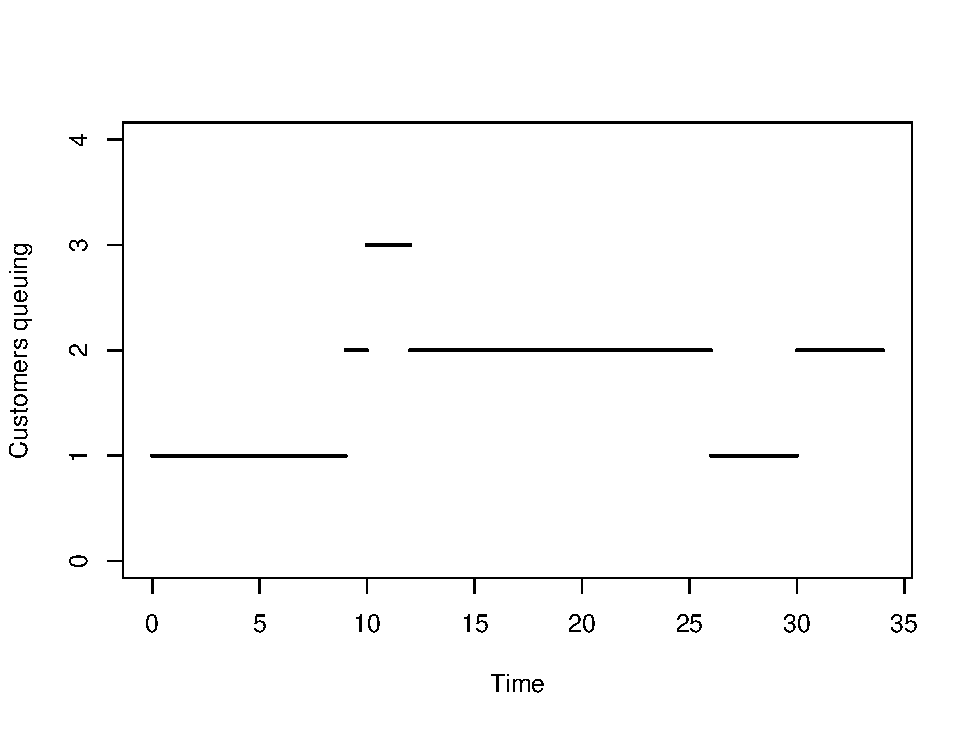
\includegraphics[width=0.8\linewidth]{SimBook_files/figure-latex/discrete-1} 

}

\caption{Example of a discrete dynamic simulation}\label{fig:discrete}
\end{figure}

Figure 1.1 further illustrates that for specific period of times the system does not change state, that is the number of customers queuing remains constant. It is therefore useless to inspect the system during those times where nothing changes. This prompts the way in which time is usually handled in dynamic discrete simulations, using the so-called \emph{next-event technique}. The model is only examined and updated when the system is due to change. These changes are usually called \emph{events}. Looking at Figure 1.1 at time zero there is an event: a customer arrives; at time nine another customer arrives; at time ten another customer arrives; at time twelve a customer is served; and so on. All these are examples of events.

\emph{Continuous} simulation models are such that the variables of interest change continuously over time. Suppose for instance a simulation model for a car journey was created where the interest is on the speed of the car throughout the journey. Then this would be a continuous simulation model. Figure 1.2 gives an illustration of this.

\begin{figure}

{\centering 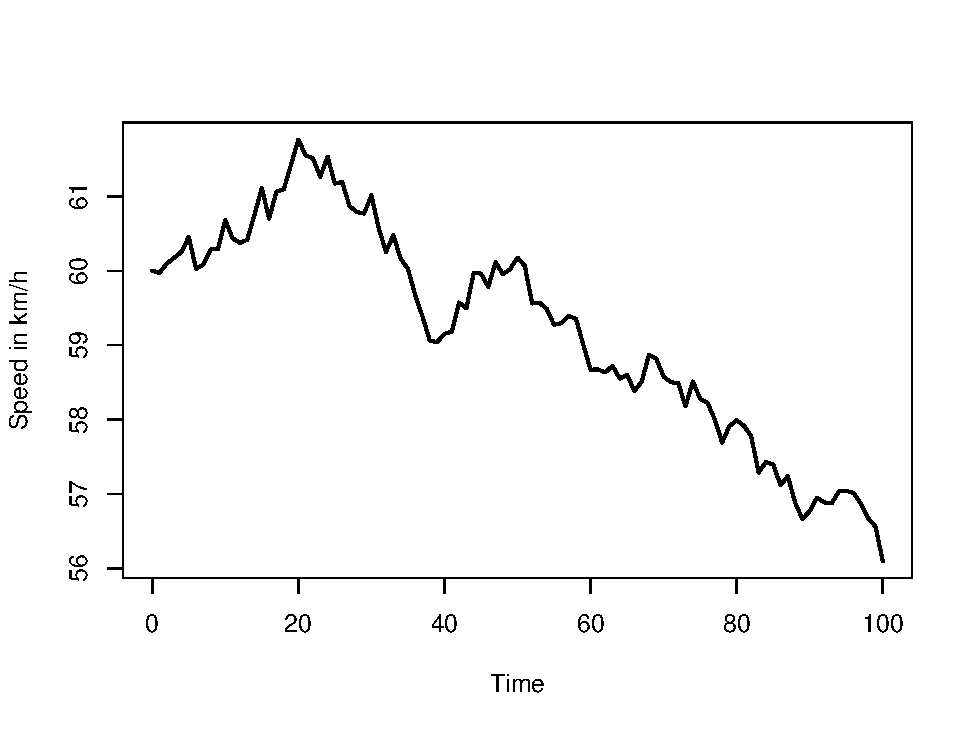
\includegraphics[width=0.8\linewidth]{SimBook_files/figure-latex/fig-cont-1} 

}

\caption{Example of a discrete dynamic simulation}\label{fig:fig-cont}
\end{figure}

In later chapters we will focus on discrete simulations, which are usually called \emph{discrete-event simulation}. Continuous simulations will not be discussed in these notes.

\hypertarget{elements-of-a-simulation-model}{%
\section{Elements of a simulation model}\label{elements-of-a-simulation-model}}

We next introduce some terminology which we will need in the following.

\hypertarget{objects-of-the-model}{%
\subsection{Objects of the model}\label{objects-of-the-model}}

There are two types of objects a simulation model is often made of:

\begin{itemize}
\item
  \emph{Entities}: individual elements of the system that are being simulated and whose behavior is being explicitly tracked. Each entity can be individually identified;
\item
  \emph{Resources}: also individual elements of the system but they are not modelled individually. They are treated as countable items whose behavior is not tracked.
\end{itemize}

Whether an element should be treated as an entity or as a resource is something that the modeller must decide and depends on the purpose of the simulation. Consider our simple donut shop. Clients will be most likely be resources since we are not really interested in what each of them do. Employees may either be considered as entities or resources: in the former case we want to track the amount of time each of them are working; in the latter the model would only be able to output an overview of how busy overall the employees are.

\hypertarget{organization-of-entities-and-resources}{%
\subsection{Organization of entities and resources}\label{organization-of-entities-and-resources}}

\begin{itemize}
\item
  \emph{Attributes}: properties of objects (that is entities and resources). This is often used to control the behavior of the object. In our donut shop an attribute may be the state of an employee: whether she is busy or available. In a more comprehensive simulation, an attribute might be the type of donut a customer will buy (for instance, chocolate, vanilla or jam).
\item
  \emph{State}: collection of variables necessary to describe the system at any time point. In our donut shop, in the simplest case the necessary variables are number of customers queuing and number of busy employees. This fully characterizes the system.
\item
  \emph{List}: collection of entites or resources ordered in some logical fashion. For instance, the customers waiting in our shop may be ordered in the so-called ``fist-come, first-served" scheme, that is customers will be served in the order they arrived in the shop.
\end{itemize}

\hypertarget{operations-of-the-objects}{%
\subsection{Operations of the objects}\label{operations-of-the-objects}}

During a simulation study, entities and resources will cooperate and therefore change state. The following terminology describe this as well as the flow of time:

\begin{itemize}
\item
  \emph{Event}: instant of time where the state of the system changes. In the donut shop suppose that there are currently two customers being served. An event is when a customer has finished being served: the number of busy employees decreases by one and there is one less customer queuing.
\item
  \emph{Activity}: a time period of specified length which is known when it begins (although its length may be random). The time an employee takes to serve a customer is an example of an activity: this may be specified in terms of a random distribution.
\item
  \emph{Delay}: duration of time of unspecified length, which is not known until it ends. This is not specified by the modeller ahead of time but is determined by the conditions of the system. Very often this is one of the desired output of a simulation. For instance, a delay is the waiting time of a customer in the queue of our donut shop.
\item
  \emph{Clock}: variable representing simulated time.
\end{itemize}

\hypertarget{the-donut-shop-example}{%
\section{The donut shop example}\label{the-donut-shop-example}}

Let's consider in more details the donut shop example and let's construct and implement our first simulation model. At this stage, you should not worry about the implementation details. These will be formalized in more details in later chapters.

Let's make some assumptions:

\begin{itemize}
\item
  the queue in the shop is possibly infinite: whenever a customer arrives she will stay in the queue independent of how many customers are already queuing and she will wait until she is served.
\item
  customers are served on a first-come, first-served basis.
\item
  there are two employees. On average they take the same time to serve a customer. Whenever an employee is free, a customer is allocated to that employee. If both employees are free, either of the two starts serving a customer.
\end{itemize}

The components of the simulation model are the following:

\begin{itemize}
\item
  \textbf{System state}: \(N_C(t)\) number of customers waiting to be served at time \(t\); \(N_E(t)\) number of employees busy at time \(t\).
\item
  \textbf{Resources}: customers and employees;
\item
  \textbf{Events}: arrival of a customer; service completion by an employee.
\item
  \textbf{Activities}: time between a customer arrival and the next; service time by an employee.
\item
  \textbf{Delay}: customers' waiting time in the queue until an employee is available.
\end{itemize}

From an abstract point of view we have now defined all components of our simulation model. Before implementing, we need to choose the length of the activities. This is usually done using common sense, intuition or historical data. Suppose for instance that the time between the arrival of customers is modeled as an Exponential distribution with parameter 1/3 (that is on average a customer arrives every three minutes) and the service time is modeled as a continuous Uniform distribution between 1 and 5 (on average a service takes three minutes).

With this information we can now implement the workings of our donut shop. It does not matter the specific code itself, we will learn about it in later chapters. At this stage it is only important to notice that we use the \texttt{simmer} package together with the functionalities of \texttt{magrittr}. We simulate our donut shop for two hours.

\begin{Shaded}
\begin{Highlighting}[]
\FunctionTok{library}\NormalTok{(simmer)}
\FunctionTok{library}\NormalTok{(magrittr)}
\FunctionTok{set.seed}\NormalTok{(}\DecValTok{2021}\NormalTok{)}

\NormalTok{env }\OtherTok{\textless{}{-}}  \FunctionTok{simmer}\NormalTok{(}\StringTok{"donut shop"}\NormalTok{)}

\NormalTok{customer }\OtherTok{\textless{}{-}} \FunctionTok{trajectory}\NormalTok{(}\StringTok{"customer"}\NormalTok{) }\SpecialCharTok{\%\textgreater{}\%} \FunctionTok{seize}\NormalTok{(}\StringTok{"employee"}\NormalTok{, }\DecValTok{1}\NormalTok{) }\SpecialCharTok{\%\textgreater{}\%}
  \FunctionTok{timeout}\NormalTok{(}\ControlFlowTok{function}\NormalTok{() }\FunctionTok{runif}\NormalTok{(}\DecValTok{1}\NormalTok{,}\DecValTok{1}\NormalTok{,}\DecValTok{5}\NormalTok{)) }\SpecialCharTok{\%\textgreater{}\%} \FunctionTok{release}\NormalTok{(}\StringTok{"employee"}\NormalTok{, }\DecValTok{1}\NormalTok{) }

\NormalTok{env }\SpecialCharTok{\%\textgreater{}\%}
  \FunctionTok{add\_resource}\NormalTok{(}\StringTok{"employee"}\NormalTok{, }\DecValTok{2}\NormalTok{) }\SpecialCharTok{\%\textgreater{}\%}
  \FunctionTok{add\_generator}\NormalTok{(}\StringTok{"customer"}\NormalTok{, customer, }\ControlFlowTok{function}\NormalTok{() }\FunctionTok{rexp}\NormalTok{(}\DecValTok{1}\NormalTok{,}\DecValTok{1}\SpecialCharTok{/}\DecValTok{3}\NormalTok{))}

\NormalTok{env }\SpecialCharTok{\%\textgreater{}\%}
  \FunctionTok{run}\NormalTok{(}\AttributeTok{until=}\DecValTok{120}\NormalTok{)}
\end{Highlighting}
\end{Shaded}

The above code creates a simulation of the donut shop for two hours. Next we report some graphical summaries that describe how the system worked.

\begin{Shaded}
\begin{Highlighting}[]
\FunctionTok{library}\NormalTok{(simmer.plot)}
\FunctionTok{library}\NormalTok{(gridExtra)}
\NormalTok{p1 }\OtherTok{\textless{}{-}} \FunctionTok{plot}\NormalTok{(}\FunctionTok{get\_mon\_resources}\NormalTok{(env), }\AttributeTok{metric =} \StringTok{"usage"}\NormalTok{, }\AttributeTok{items =} \StringTok{"server"}\NormalTok{,}\AttributeTok{step =}\NormalTok{ T)}
\NormalTok{p2 }\OtherTok{\textless{}{-}} \FunctionTok{plot}\NormalTok{(}\FunctionTok{get\_mon\_arrivals}\NormalTok{(env), }\AttributeTok{metric =} \StringTok{"waiting\_time"}\NormalTok{)}

\FunctionTok{grid.arrange}\NormalTok{(p1,p2,}\AttributeTok{ncol=}\DecValTok{2}\NormalTok{)}
\end{Highlighting}
\end{Shaded}

\begin{figure}

{\centering 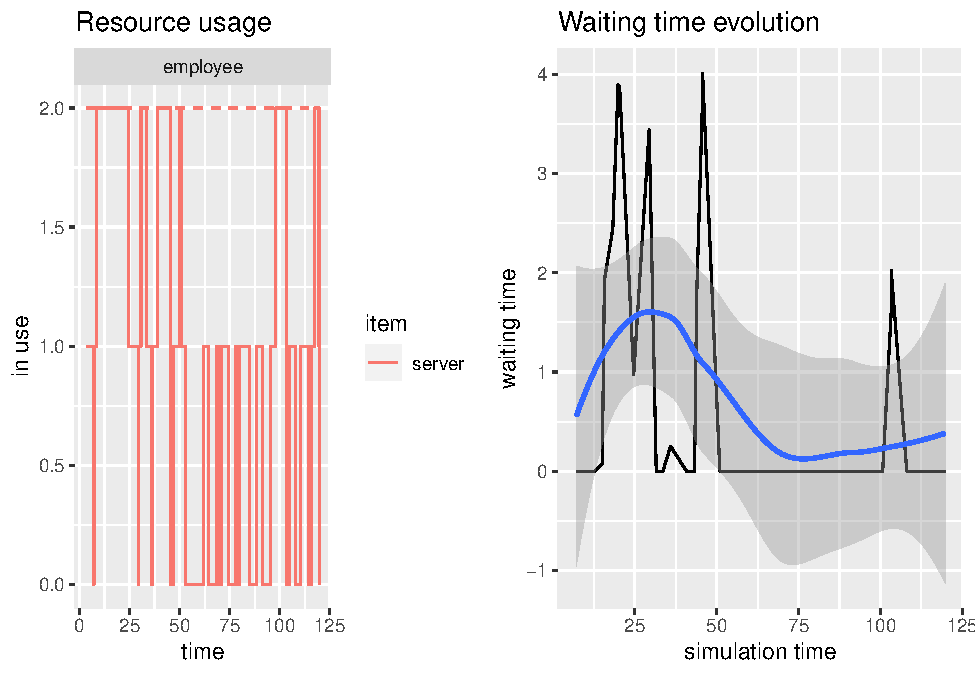
\includegraphics{SimBook_files/figure-latex/donut-1} 

}

\caption{Graphical summaries from the simulation of the donut shop}\label{fig:donut}
\end{figure}

The left plot in Figure 1.3 reports the number of busy employees busy throughout the simulation. We can observe that often no employees were busy, but sometimes both of them are busy. The right plot in Figure 1.3 reports the waiting time of customers throughout the simulation. Most often customers do not wait in our shop and the largest waiting time is of about four minutes.

Some observations:

\begin{itemize}
\item
  this is the result of a single simulation where inputs are random and described by a random variable (for instance, Poisson and Uniform). If we were to run the simulation again we would observe different results.
\item
  given that we have built the simulation model, it is straightforward to change some of the inputs and observe the results under different conditions. For instance, we could investigate what would happen if we had only one employee. We could also investigate the use of different input parameters for the customer arrival times and the service times.
\end{itemize}

\hypertarget{simulating-a-little-health-center}{%
\section{Simulating a little health center}\label{simulating-a-little-health-center}}

Consider now a slightly more complex example where we want to simulate the workings of a little health center. Patients arrive at the health center and are first visited by a nurse. Once they are visited by the nurse they have an actual consultation with a doctor. Once they are finished with the doctor, they meet the administrative staff to schedule a follow-up appointment.

We make the following assumptions:

\begin{itemize}
\item
  as before we assume queues to be infinite and that patients do not leave the health center until they are served by the administrative staff;
\item
  at all steps patients are visited using a first-come, first-served basis
\item
  the health center has one nurse, two doctors and one administrative staff. The two doctors take on average the same time to visit a patient.
\end{itemize}

The components of the simulation model are the following:

\begin{itemize}
\item
  \textbf{System state}:

  \begin{itemize}
  \item
    \(Q_N(t)\): number of patients queuing to see the nurse;
  \item
    \(Q_D(t)\): number of patients queing to see a doctor;
  \item
    \(Q_A(t)\): number of patients queuing to see the staff;
  \item
    \(N_N(t)\): number of nurses available to visit patients;
  \item
    \(N_D(t)\): number of doctors available to visit patients;
  \item
    \(N_A(t)\): number of administrative staff available to visit patients.
  \end{itemize}
\item
  \textbf{Resources}: patients, nurses, doctors and administrative staff;
\item
  \textbf{Events}: arrival of a patient, completion of nurse's visit, completation of doctor's visit, completion of administrative staff's visit.
\item
  \textbf{Activities}: time between the arrival of a patient and the next, visit's times of nurses, doctors and admin staff.
\item
  \textbf{Delay}: customers' waiting time for nurses, doctors and administrative staff
\end{itemize}

We further assume the following activities:

\begin{itemize}
\item
  Nurse visit times follow a Normal distribution with mean 15 and variance 1;
\item
  Doctor visit times follow a Normal distribution with mean 20 and variance 1;
\item
  Administrative staff visit times follow a Normal distribution with mean 5 and variance 1;
\item
  Time between the arrival of patients is modeled as a Normal with mean 10 and variance 4.
\end{itemize}

The model above can be implemented using the following code (we run the simulation for four hours). Again do not worry about it now!

\begin{Shaded}
\begin{Highlighting}[]
\FunctionTok{set.seed}\NormalTok{(}\DecValTok{2021}\NormalTok{)}
\NormalTok{env }\OtherTok{\textless{}{-}} \FunctionTok{simmer}\NormalTok{(}\StringTok{"HealthCenter"}\NormalTok{)}

\NormalTok{patient }\OtherTok{\textless{}{-}} \FunctionTok{trajectory}\NormalTok{(}\StringTok{"patients\textquotesingle{} path"}\NormalTok{) }\SpecialCharTok{\%\textgreater{}\%}
  \FunctionTok{seize}\NormalTok{(}\StringTok{"nurse"}\NormalTok{, }\DecValTok{1}\NormalTok{) }\SpecialCharTok{\%\textgreater{}\%}
  \FunctionTok{timeout}\NormalTok{(}\ControlFlowTok{function}\NormalTok{() }\FunctionTok{rnorm}\NormalTok{(}\DecValTok{1}\NormalTok{, }\DecValTok{15}\NormalTok{)) }\SpecialCharTok{\%\textgreater{}\%}
  \FunctionTok{release}\NormalTok{(}\StringTok{"nurse"}\NormalTok{, }\DecValTok{1}\NormalTok{) }\SpecialCharTok{\%\textgreater{}\%}
  \FunctionTok{seize}\NormalTok{(}\StringTok{"doctor"}\NormalTok{, }\DecValTok{1}\NormalTok{) }\SpecialCharTok{\%\textgreater{}\%}
  \FunctionTok{timeout}\NormalTok{(}\ControlFlowTok{function}\NormalTok{() }\FunctionTok{rnorm}\NormalTok{(}\DecValTok{1}\NormalTok{, }\DecValTok{20}\NormalTok{)) }\SpecialCharTok{\%\textgreater{}\%}
  \FunctionTok{release}\NormalTok{(}\StringTok{"doctor"}\NormalTok{, }\DecValTok{1}\NormalTok{) }\SpecialCharTok{\%\textgreater{}\%}
  \FunctionTok{seize}\NormalTok{(}\StringTok{"administration"}\NormalTok{, }\DecValTok{1}\NormalTok{) }\SpecialCharTok{\%\textgreater{}\%}
  \FunctionTok{timeout}\NormalTok{(}\ControlFlowTok{function}\NormalTok{() }\FunctionTok{rnorm}\NormalTok{(}\DecValTok{1}\NormalTok{, }\DecValTok{5}\NormalTok{)) }\SpecialCharTok{\%\textgreater{}\%}
  \FunctionTok{release}\NormalTok{(}\StringTok{"administration"}\NormalTok{, }\DecValTok{1}\NormalTok{)}

\NormalTok{env }\SpecialCharTok{\%\textgreater{}\%}
  \FunctionTok{add\_resource}\NormalTok{(}\StringTok{"nurse"}\NormalTok{, }\DecValTok{1}\NormalTok{) }\SpecialCharTok{\%\textgreater{}\%}
  \FunctionTok{add\_resource}\NormalTok{(}\StringTok{"doctor"}\NormalTok{, }\DecValTok{2}\NormalTok{) }\SpecialCharTok{\%\textgreater{}\%}
  \FunctionTok{add\_resource}\NormalTok{(}\StringTok{"administration"}\NormalTok{, }\DecValTok{1}\NormalTok{) }\SpecialCharTok{\%\textgreater{}\%}
  \FunctionTok{add\_generator}\NormalTok{(}\StringTok{"patient"}\NormalTok{, patient, }\ControlFlowTok{function}\NormalTok{() }\FunctionTok{rnorm}\NormalTok{(}\DecValTok{1}\NormalTok{, }\DecValTok{10}\NormalTok{, }\DecValTok{2}\NormalTok{))}

\NormalTok{env }\SpecialCharTok{\%\textgreater{}\%} \FunctionTok{run}\NormalTok{(}\DecValTok{240}\NormalTok{)}
\end{Highlighting}
\end{Shaded}

Let's look at some summary statistics.

\begin{Shaded}
\begin{Highlighting}[]
\FunctionTok{plot}\NormalTok{(}\FunctionTok{get\_mon\_resources}\NormalTok{(env), }\AttributeTok{metric =} \StringTok{"utilization"}\NormalTok{)}
\end{Highlighting}
\end{Shaded}

\begin{figure}

{\centering 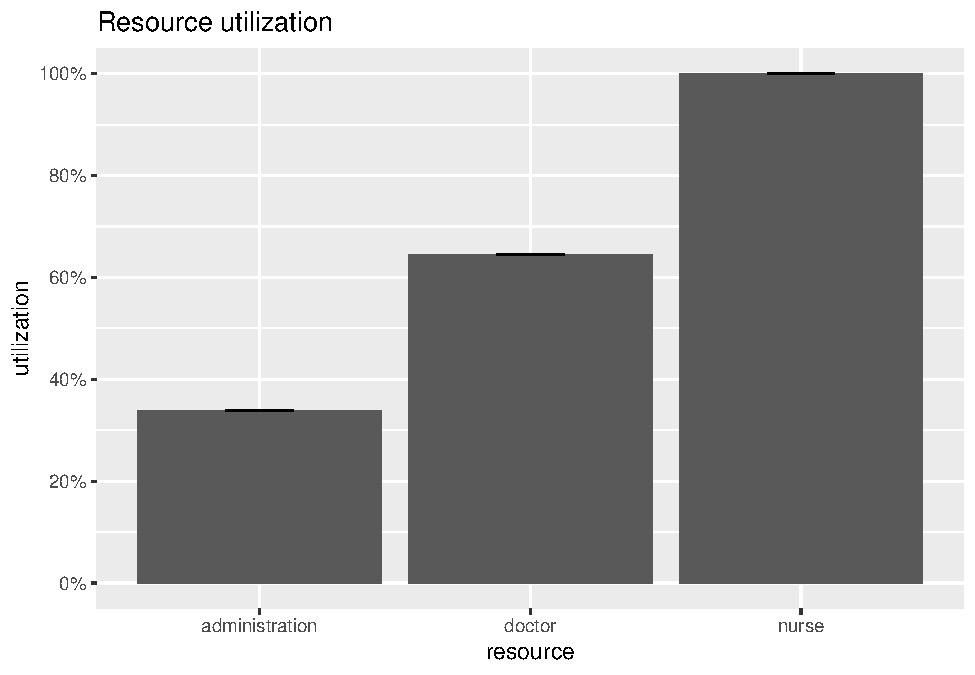
\includegraphics{SimBook_files/figure-latex/unnamed-chunk-4-1} 

}

\caption{Utilization of the resources in the health center}\label{fig:unnamed-chunk-4}
\end{figure}

Figure 1.4 shows the utilization of the different resources in the system. Nurses are most busy, doctors are overall fairly available, whilst the administration is more than half of the time available.

\begin{Shaded}
\begin{Highlighting}[]
\FunctionTok{plot}\NormalTok{(}\FunctionTok{get\_mon\_resources}\NormalTok{(env), }\AttributeTok{metric =} \StringTok{"usage"}\NormalTok{, }\AttributeTok{item =} \StringTok{"server"}\NormalTok{)}
\end{Highlighting}
\end{Shaded}

\begin{figure}

{\centering 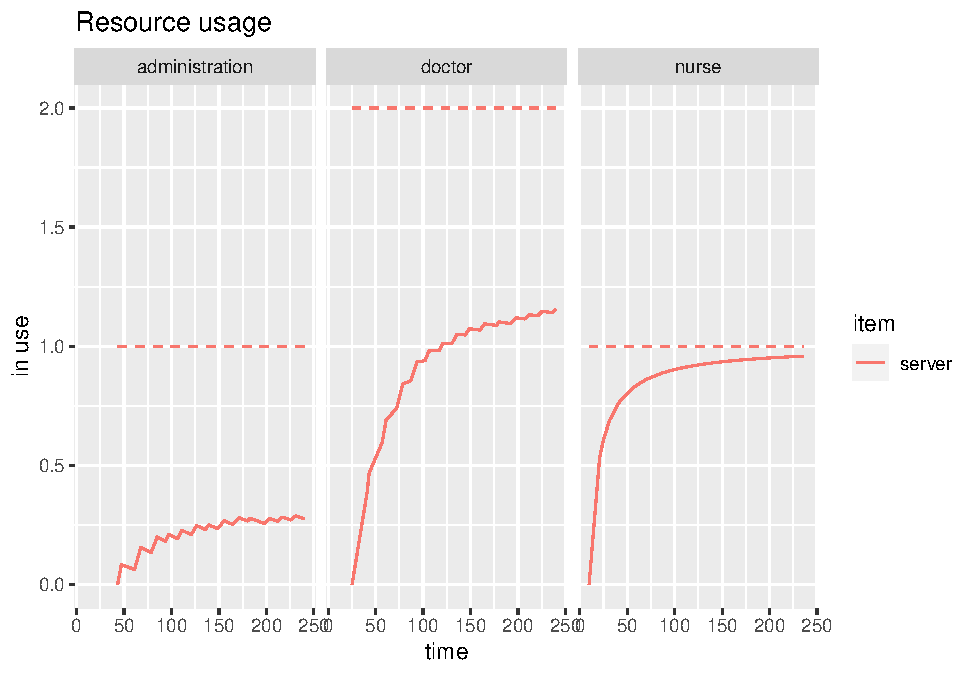
\includegraphics{SimBook_files/figure-latex/unnamed-chunk-5-1} 

}

\caption{Usage of the resources in the health center}\label{fig:unnamed-chunk-5}
\end{figure}

Figure 1.5 confirms this. We see that the usage of nurses is almost 1, whilst for doctors and administrative staff we are below the number of doctors and staff available.

\begin{Shaded}
\begin{Highlighting}[]
\FunctionTok{plot}\NormalTok{(}\FunctionTok{get\_mon\_arrivals}\NormalTok{(env), }\AttributeTok{metric =} \StringTok{"flow\_time"}\NormalTok{)}
\end{Highlighting}
\end{Shaded}

\begin{figure}

{\centering 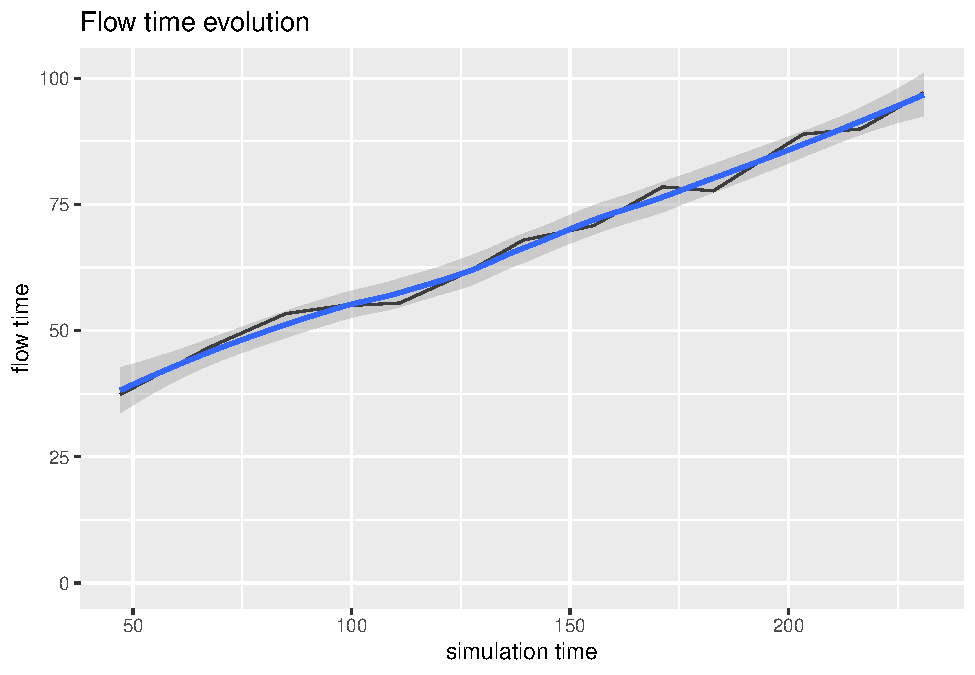
\includegraphics{SimBook_files/figure-latex/unnamed-chunk-6-1} 

}

\caption{Time spent in the health center}\label{fig:unnamed-chunk-6}
\end{figure}

Last Figure 1.6 reports the average time spent by patients in the health center. We can see that as the simulation clock increases, patients spend more time in the health center. From the previous plots, we can deduce that in general patients wait for the nurse, who has been busy all the time during the simulation.

\hypertarget{whats-next}{%
\section{What's next}\label{whats-next}}

The previous examples should have given you an idea of what a simulation model is and what you will be able to implement by the end of the course. However, it will take some time before we get to actually simulate systems. There are various skills that you will need to learn or revise before being able to implement simulation in R yourself. Specifically:

\begin{itemize}
\item
  first we will review the basics of R programming;
\item
  we will then review basic elements of probability and statistics;
\item
  we will discuss how randomness is implemented in programming languages and in R;
\item
  at this stage you will be able to implement your first simple simulations. In particular we will start with static simulation, also called \emph{Monte Carlo} simulation
\item
  we will then look at dynamic simulations as in the previous examples.
\end{itemize}

\hypertarget{r-programming}{%
\chapter{R programming}\label{r-programming}}

R is a programming language most commonly used within the statistical and machine learning community. This chapter will review some of the elements of R programming that will be used in later chapters. Do not expect this chapter to be exhaustive or self-contained. It is intended to give a quick refresh of R for users that have at least some experience with this programming language. There are many topics and concepts which are fundamental but will not be reviewed in this chapter. However, you should aim to master the topics included in this chapter since they will appear again later on in these notes. There are many other resources if you want to have a more in-depth look into R programming.

\begin{itemize}
\item
  The books of Hadley Wickham are surely a great starting point and are all available \href{http://hadley.nz/}{here}.
\item
  If you are unsure on how to do something with R, Google it!!! The community of R users is so wide that surely someone else has already asked your same question.
\item
  The R help is extremely useful and comprehensive. If you want to know more about a function, suppose it is called function, you can type \texttt{?function}.
\end{itemize}

\hypertarget{why-r}{%
\section{Why R?}\label{why-r}}

As mentioned in the previous chapter, simulation is very often applied in many areas, for instance management science and engineering. Often a simulation is carried out using an Excel spreadsheet or using a specialised software whose only purpose is creating simulations. Historically, R has not been at the forefront of the implementation of simulation models, in particular of discrete-event simulations. Only recently, R packages implementing discrete-event simulation have appeared, most importantly the \texttt{simmer} R package that you will learn using in later chapters.

These notes are intended to provide a unique view of simulation with specific implementation in the R programming language. Some of the strenght of R are:

\begin{itemize}
\item
  it is free, open-source and available in all major operating systems;
\item
  the community of R users is huge, with many forums, sites and resources that give you practical support in developing your own code;
\item
  a massive set of add-on packages to increase the capabalities of the basic R environment;
\item
  functions to perform state-of-the-art statistical and machine-learning methods. Researchers sometimes create an associated R package to any article they publish so for others to use their methods;
\item
  the integrated development environment RStudio provides a user-friendly environment to make the R programming experience more pleasing;
\item
  powerful communication tools to create documents and presentations embedding R code and R output. As a matter of fact this very book is created in R!!!!
\end{itemize}

\hypertarget{r-basics}{%
\section{R basics}\label{r-basics}}

So let's get started with R programming!

\hypertarget{r-as-a-calculator}{%
\subsection{R as a calculator}\label{r-as-a-calculator}}

In its most basic usage, we can use R as a calculator. Basic algebraic operations can be carried out as you would expect. The symbol \texttt{+} is for sum, \texttt{-} for subtraction, \texttt{*} for multiplication and \texttt{/} for division. Here are some examples:

\begin{Shaded}
\begin{Highlighting}[]
\DecValTok{4} \SpecialCharTok{+} \DecValTok{2}
\end{Highlighting}
\end{Shaded}

\begin{verbatim}
## [1] 6
\end{verbatim}

\begin{Shaded}
\begin{Highlighting}[]
\DecValTok{4} \SpecialCharTok{{-}} \DecValTok{2}
\end{Highlighting}
\end{Shaded}

\begin{verbatim}
## [1] 2
\end{verbatim}

\begin{Shaded}
\begin{Highlighting}[]
\DecValTok{4} \SpecialCharTok{*} \DecValTok{2}
\end{Highlighting}
\end{Shaded}

\begin{verbatim}
## [1] 8
\end{verbatim}

\begin{Shaded}
\begin{Highlighting}[]
\DecValTok{5} \SpecialCharTok{/} \DecValTok{2}
\end{Highlighting}
\end{Shaded}

\begin{verbatim}
## [1] 2.5
\end{verbatim}

\hypertarget{variable-assignment}{%
\subsection{Variable assignment}\label{variable-assignment}}

In R the symbol \texttt{\textless{}-} is used to assign a quantity to a variable. For instance, \texttt{a\ \textless{}-\ 4} assigns the number \texttt{4} to the variable \texttt{a} and \texttt{b\ \textless{}-\ 3} assigns the number \texttt{3} to \texttt{b}. It is much more common to work with variables in programming. Basic operations can then be performed over variables.

\begin{Shaded}
\begin{Highlighting}[]
\NormalTok{a }\OtherTok{\textless{}{-}} \DecValTok{4}
\NormalTok{b }\OtherTok{\textless{}{-}} \DecValTok{3}
\NormalTok{a }\SpecialCharTok{+}\NormalTok{ b}
\end{Highlighting}
\end{Shaded}

\begin{verbatim}
## [1] 7
\end{verbatim}

\begin{Shaded}
\begin{Highlighting}[]
\NormalTok{a }\SpecialCharTok{{-}}\NormalTok{ b}
\end{Highlighting}
\end{Shaded}

\begin{verbatim}
## [1] 1
\end{verbatim}

Notice for example that the code \texttt{a\ \textless{}-\ 4} does not show us the value of the variable \texttt{a}. It only creates this assignment. If we want to print the value of a variable, we have to explictly type the name of the variable.

\begin{Shaded}
\begin{Highlighting}[]
\NormalTok{a}
\end{Highlighting}
\end{Shaded}

\begin{verbatim}
## [1] 4
\end{verbatim}

\hypertarget{data-types}{%
\subsection{Data types}\label{data-types}}

In the previous examples we worked with numbers, but variables could be assigned other types of information. There are four basic types:

\begin{itemize}
\item
  \emph{Logicals} or \emph{Booleans}: corresponding to \texttt{TRUE} and \texttt{FALSE}, also abbreviated as \texttt{T} and \texttt{F} respectively;
\item
  \emph{Doubles}: real numbers;
\item
  \emph{Characters}: strings of text surrounded by \texttt{"} (for example \texttt{"hi"}) or by \texttt{\textquotesingle{}} (for example `by');
\item
  \emph{Integers}: integer numbers. If you type an integer in R, as before 3 or 4, it will usually be stored as a double unless explicitly defined.
\end{itemize}

Examples:

\begin{Shaded}
\begin{Highlighting}[]
\NormalTok{a }\OtherTok{\textless{}{-}} \ConstantTok{TRUE}
\NormalTok{a}
\end{Highlighting}
\end{Shaded}

\begin{verbatim}
## [1] TRUE
\end{verbatim}

\begin{Shaded}
\begin{Highlighting}[]
\NormalTok{b }\OtherTok{\textless{}{-}} \StringTok{"hello"}
\NormalTok{b}
\end{Highlighting}
\end{Shaded}

\begin{verbatim}
## [1] "hello"
\end{verbatim}

\hypertarget{vectors}{%
\subsection{Vectors}\label{vectors}}

In all previous examples the variables included one element only. More generally we can define sequences of elements or so-called \emph{vectors}. They can be defined with the command \texttt{c}, which stands for combine.

\begin{Shaded}
\begin{Highlighting}[]
\NormalTok{vec }\OtherTok{\textless{}{-}} \FunctionTok{c}\NormalTok{(}\DecValTok{1}\NormalTok{,}\DecValTok{3}\NormalTok{,}\DecValTok{5}\NormalTok{,}\DecValTok{7}\NormalTok{)}
\NormalTok{vec}
\end{Highlighting}
\end{Shaded}

\begin{verbatim}
## [1] 1 3 5 7
\end{verbatim}

So \texttt{vec} includes the sequence of numbers 1, 3, 5, 7. Notice that a vector can only include one data type. Consider the following:

\begin{Shaded}
\begin{Highlighting}[]
\NormalTok{vec }\OtherTok{\textless{}{-}} \FunctionTok{c}\NormalTok{(}\DecValTok{1}\NormalTok{, }\StringTok{"hello"}\NormalTok{, }\ConstantTok{TRUE}\NormalTok{)}
\NormalTok{vec}
\end{Highlighting}
\end{Shaded}

\begin{verbatim}
## [1] "1"     "hello" "TRUE"
\end{verbatim}

We created a variable \texttt{vec} where the first entry is a number, then a character string, then a Boolean. When we print \texttt{vec}, we get that its elements are \texttt{"1"}, \texttt{"hello"} and \texttt{"TRUE"}: it has transformed the number \texttt{1} into the string \texttt{"1"} and the Boolean \texttt{TRUE} into \texttt{"TRUE"}.

\hypertarget{matrices}{%
\subsection{Matrices}\label{matrices}}

Matrices are tables of elements that are organized in rows and columns. You can think of them as an arrangement of vectors into a table. Matrices must have the same data type in all its entries, as for vectors. Matrices can be constructed in multiple ways. One way is by stacking vectors into a matrix row-by-row with the command \texttt{rbind}. Consider the following example.

\begin{Shaded}
\begin{Highlighting}[]
\NormalTok{row1 }\OtherTok{\textless{}{-}} \FunctionTok{c}\NormalTok{(}\DecValTok{1}\NormalTok{,}\DecValTok{2}\NormalTok{,}\DecValTok{3}\NormalTok{)}
\NormalTok{row2 }\OtherTok{\textless{}{-}} \FunctionTok{c}\NormalTok{(}\DecValTok{4}\NormalTok{,}\DecValTok{5}\NormalTok{,}\DecValTok{6}\NormalTok{)}
\NormalTok{row3 }\OtherTok{\textless{}{-}} \FunctionTok{c}\NormalTok{(}\DecValTok{7}\NormalTok{,}\DecValTok{8}\NormalTok{,}\DecValTok{9}\NormalTok{)}
\NormalTok{mat }\OtherTok{\textless{}{-}} \FunctionTok{rbind}\NormalTok{(row1,row2,row3)}
\NormalTok{mat}
\end{Highlighting}
\end{Shaded}

\begin{verbatim}
##      [,1] [,2] [,3]
## row1    1    2    3
## row2    4    5    6
## row3    7    8    9
\end{verbatim}

So first we created vectors \texttt{row1\ =\ (1,2,3)}, \texttt{row2\ =\ (4,5,6)} and \texttt{row3\ =\ (7,8,9)} and then organizing them together into the matrix \texttt{mat}.

The following code follows the same procedure but now organizes vectors by columns instead using the command \texttt{cbind}.

\begin{Shaded}
\begin{Highlighting}[]
\NormalTok{col1 }\OtherTok{\textless{}{-}} \FunctionTok{c}\NormalTok{(}\DecValTok{1}\NormalTok{,}\DecValTok{2}\NormalTok{,}\DecValTok{3}\NormalTok{)}
\NormalTok{col2 }\OtherTok{\textless{}{-}} \FunctionTok{c}\NormalTok{(}\DecValTok{4}\NormalTok{,}\DecValTok{5}\NormalTok{,}\DecValTok{6}\NormalTok{)}
\NormalTok{col3 }\OtherTok{\textless{}{-}} \FunctionTok{c}\NormalTok{(}\DecValTok{7}\NormalTok{,}\DecValTok{8}\NormalTok{,}\DecValTok{9}\NormalTok{)}
\NormalTok{mat }\OtherTok{\textless{}{-}} \FunctionTok{cbind}\NormalTok{(col1,col2,col3)}
\NormalTok{mat}
\end{Highlighting}
\end{Shaded}

\begin{verbatim}
##      col1 col2 col3
## [1,]    1    4    7
## [2,]    2    5    8
## [3,]    3    6    9
\end{verbatim}

Last, there is also a command called \texttt{matrix} to create a matrix. It takes a vector, defined using the command \texttt{c} and stores its entries into a matrix of \texttt{nrow} rows and \texttt{ncol} columns. Consider the following example.

\begin{Shaded}
\begin{Highlighting}[]
\NormalTok{vec }\OtherTok{\textless{}{-}} \FunctionTok{c}\NormalTok{(}\DecValTok{1}\NormalTok{,}\DecValTok{2}\NormalTok{,}\DecValTok{3}\NormalTok{,}\DecValTok{4}\NormalTok{,}\DecValTok{5}\NormalTok{,}\DecValTok{6}\NormalTok{,}\DecValTok{7}\NormalTok{,}\DecValTok{8}\NormalTok{,}\DecValTok{9}\NormalTok{)}
\NormalTok{mat }\OtherTok{\textless{}{-}} \FunctionTok{matrix}\NormalTok{(vec, }\AttributeTok{nrow =} \DecValTok{3}\NormalTok{, }\AttributeTok{ncol =} \DecValTok{3}\NormalTok{)}
\NormalTok{mat}
\end{Highlighting}
\end{Shaded}

\begin{verbatim}
##      [,1] [,2] [,3]
## [1,]    1    4    7
## [2,]    2    5    8
## [3,]    3    6    9
\end{verbatim}

So first we created a vector \texttt{vec} with numbers from 1 to 9 and then stored them in a matrix with 3 rows and 3 columns. Number are stored by column: the first element of \texttt{vec} is in entry (1,1), the second element of \texttt{vec} is in entry (2,1), and so on.

\hypertarget{dataframes}{%
\subsection{Dataframes}\label{dataframes}}

Dataframes are very similar as matrices, they are tables organized in rows and columns. However, different to matrices they can have columns with different data types. They can be created with the command \texttt{data.frame}.

\begin{Shaded}
\begin{Highlighting}[]
\NormalTok{data }\OtherTok{\textless{}{-}} \FunctionTok{data.frame}\NormalTok{(}\AttributeTok{X1 =} \FunctionTok{c}\NormalTok{(}\DecValTok{1}\NormalTok{,}\DecValTok{2}\NormalTok{,}\DecValTok{3}\NormalTok{), }\AttributeTok{X2 =} \FunctionTok{c}\NormalTok{(}\ConstantTok{TRUE}\NormalTok{,}\ConstantTok{FALSE}\NormalTok{,}\ConstantTok{FALSE}\NormalTok{),}
                   \AttributeTok{X3 =} \FunctionTok{c}\NormalTok{(}\StringTok{"male"}\NormalTok{,}\StringTok{"male"}\NormalTok{,}\StringTok{"female"}\NormalTok{))}
\NormalTok{data}
\end{Highlighting}
\end{Shaded}

\begin{verbatim}
##   X1    X2     X3
## 1  1  TRUE   male
## 2  2 FALSE   male
## 3  3 FALSE female
\end{verbatim}

The dataframe \texttt{data} includes three columns: the first column \texttt{X1} of numbers, the second column \texttt{X2} of Boolean and the third column \texttt{X3} of characters. Dataframes are the objects that are most commonly used in real world data analysis.

\hypertarget{null-and-na}{%
\subsection{\texorpdfstring{\texttt{NULL} and \texttt{NA}}{NULL and NA}}\label{null-and-na}}

The expression \texttt{NA} is used in R to denote a missing value. Consider the following example.

\begin{Shaded}
\begin{Highlighting}[]
\NormalTok{vec }\OtherTok{\textless{}{-}} \FunctionTok{c}\NormalTok{(}\DecValTok{3}\NormalTok{, }\ConstantTok{NA}\NormalTok{, }\DecValTok{5}\NormalTok{)}
\NormalTok{vec}
\end{Highlighting}
\end{Shaded}

\begin{verbatim}
## [1]  3 NA  5
\end{verbatim}

Although the second element of \texttt{vec} is the expression \texttt{NA}, R recognizes that it is used for missing value and therefore the elements 3 and 5 are still considered numbers: indeed they are not printed as \texttt{"3"} and \texttt{"5"}.

\texttt{NULL} is an additional datatype. This can have various uses. For instance, it is associated to a vector with no entries.

\begin{Shaded}
\begin{Highlighting}[]
\FunctionTok{c}\NormalTok{()}
\end{Highlighting}
\end{Shaded}

\begin{verbatim}
## NULL
\end{verbatim}

\hypertarget{accessing-and-manipulating-variables}{%
\section{Accessing and manipulating variables}\label{accessing-and-manipulating-variables}}

Now that we have described the main objects we will work with in R, we can discuss how to access specific information.

\hypertarget{accessing-a-single-element}{%
\subsection{Accessing a single element}\label{accessing-a-single-element}}

Given a vector \texttt{vec} we can access its i-th entry with \texttt{vec{[}i{]}}.

\begin{Shaded}
\begin{Highlighting}[]
\NormalTok{vec }\OtherTok{\textless{}{-}} \FunctionTok{c}\NormalTok{(}\DecValTok{1}\NormalTok{,}\DecValTok{3}\NormalTok{,}\DecValTok{5}\NormalTok{)}
\NormalTok{vec[}\DecValTok{2}\NormalTok{]}
\end{Highlighting}
\end{Shaded}

\begin{verbatim}
## [1] 3
\end{verbatim}

For a matrix or a dataframe we need to specify the associated row and column. If we have a matrix \texttt{mat} we can access the element in entry (i,j) with \texttt{mat{[}i,j{]}}.

\begin{Shaded}
\begin{Highlighting}[]
\NormalTok{mat }\OtherTok{\textless{}{-}} \FunctionTok{matrix}\NormalTok{(}\FunctionTok{c}\NormalTok{(}\DecValTok{1}\NormalTok{,}\DecValTok{2}\NormalTok{,}\DecValTok{3}\NormalTok{,}\DecValTok{4}\NormalTok{,}\DecValTok{5}\NormalTok{,}\DecValTok{6}\NormalTok{,}\DecValTok{7}\NormalTok{,}\DecValTok{8}\NormalTok{,}\DecValTok{9}\NormalTok{), }\AttributeTok{ncol=}\DecValTok{3}\NormalTok{, }\AttributeTok{nrow =}\DecValTok{3}\NormalTok{)}
\NormalTok{mat[}\DecValTok{1}\NormalTok{,}\DecValTok{3}\NormalTok{]}
\end{Highlighting}
\end{Shaded}

\begin{verbatim}
## [1] 7
\end{verbatim}

\hypertarget{acessing-multiple-entries}{%
\subsection{Acessing multiple entries}\label{acessing-multiple-entries}}

To access multiple entries we can on the other hand define a vector of indexes of the elements we want to access. Consider the following examples:

\begin{Shaded}
\begin{Highlighting}[]
\NormalTok{vec }\OtherTok{\textless{}{-}} \FunctionTok{c}\NormalTok{(}\DecValTok{1}\NormalTok{,}\DecValTok{3}\NormalTok{,}\DecValTok{5}\NormalTok{)}
\NormalTok{vec[}\FunctionTok{c}\NormalTok{(}\DecValTok{1}\NormalTok{,}\DecValTok{2}\NormalTok{)]}
\end{Highlighting}
\end{Shaded}

\begin{verbatim}
## [1] 1 3
\end{verbatim}

The above code accesses the first two entries of the vector \texttt{vec}. To do this we had to define a vector using \texttt{c(1,2)} stating the entries we wanted to look at. For matrices consider:

\begin{Shaded}
\begin{Highlighting}[]
\NormalTok{mat }\OtherTok{\textless{}{-}} \FunctionTok{matrix}\NormalTok{(}\FunctionTok{c}\NormalTok{(}\DecValTok{1}\NormalTok{,}\DecValTok{2}\NormalTok{,}\DecValTok{3}\NormalTok{,}\DecValTok{4}\NormalTok{,}\DecValTok{5}\NormalTok{,}\DecValTok{6}\NormalTok{,}\DecValTok{7}\NormalTok{,}\DecValTok{8}\NormalTok{,}\DecValTok{9}\NormalTok{), }\AttributeTok{ncol=}\DecValTok{3}\NormalTok{, }\AttributeTok{nrow =}\DecValTok{3}\NormalTok{)}
\NormalTok{mat[}\FunctionTok{c}\NormalTok{(}\DecValTok{1}\NormalTok{,}\DecValTok{2}\NormalTok{),}\FunctionTok{c}\NormalTok{(}\DecValTok{2}\NormalTok{,}\DecValTok{3}\NormalTok{)]}
\end{Highlighting}
\end{Shaded}

\begin{verbatim}
##      [,1] [,2]
## [1,]    4    7
## [2,]    5    8
\end{verbatim}

The syntax is very similar as before. We defined to index vectors, one for the rows and one for columns. The two statements \texttt{c(1,2)} and \texttt{c(2,3)} are separated by a comma to denote that the first selects the first and second row, whilst the second selects the second and third column.

If one wants to access full rows or full columns, the argument associated to rows or columns is left blank. Consider the following examples.

\begin{Shaded}
\begin{Highlighting}[]
\NormalTok{mat }\OtherTok{\textless{}{-}} \FunctionTok{matrix}\NormalTok{(}\FunctionTok{c}\NormalTok{(}\DecValTok{1}\NormalTok{,}\DecValTok{2}\NormalTok{,}\DecValTok{3}\NormalTok{,}\DecValTok{4}\NormalTok{,}\DecValTok{5}\NormalTok{,}\DecValTok{6}\NormalTok{,}\DecValTok{7}\NormalTok{,}\DecValTok{8}\NormalTok{,}\DecValTok{9}\NormalTok{), }\AttributeTok{ncol=}\DecValTok{3}\NormalTok{, }\AttributeTok{nrow =}\DecValTok{3}\NormalTok{)}
\NormalTok{mat[}\DecValTok{1}\NormalTok{,]}
\end{Highlighting}
\end{Shaded}

\begin{verbatim}
## [1] 1 4 7
\end{verbatim}

\begin{Shaded}
\begin{Highlighting}[]
\NormalTok{mat[,}\FunctionTok{c}\NormalTok{(}\DecValTok{1}\NormalTok{,}\DecValTok{2}\NormalTok{)]}
\end{Highlighting}
\end{Shaded}

\begin{verbatim}
##      [,1] [,2]
## [1,]    1    4
## [2,]    2    5
## [3,]    3    6
\end{verbatim}

The code \texttt{mat{[}1,{]}} selects the first full row of \texttt{mat}. The code \texttt{mat{[},c(1,2){]}} selects the first and second column of \texttt{mat}. Notice that the comma has always to be included!

To access multiple entries it is often useful to define sequences of number quickly. The following command defines the sequence of integer numbers from 1 to 9.

\begin{Shaded}
\begin{Highlighting}[]
\DecValTok{1}\SpecialCharTok{:}\DecValTok{9}
\end{Highlighting}
\end{Shaded}

\begin{verbatim}
## [1] 1 2 3 4 5 6 7 8 9
\end{verbatim}

More generally, one can define sequences of numbers using \texttt{seq} (see \texttt{?seq}).

\hypertarget{accessing-entries-with-logical-operators}{%
\subsection{Accessing entries with logical operators}\label{accessing-entries-with-logical-operators}}

If we want to access elements of an object based on a condition it is often easier to use logical operators. This means comparing entries using the comparisons you would usually use in mathematical reasoning, for instance being equal to, or being larger to. The syntax is as follows:

\begin{itemize}
\item
  \texttt{==} to check equality (notice the two equal signs)
\item
  \texttt{!=} to check non-equality
\item
  \texttt{\textgreater{}} bigger to
\item
  \texttt{\textgreater{}=} bigger or equal to
\item
  \texttt{\textless{}} less to
\item
  \texttt{\textless{}=} less or equal to
\end{itemize}

Let's see some examples.

\begin{Shaded}
\begin{Highlighting}[]
\NormalTok{vec }\OtherTok{\textless{}{-}} \FunctionTok{c}\NormalTok{(}\DecValTok{2}\NormalTok{,}\DecValTok{3}\NormalTok{,}\DecValTok{4}\NormalTok{,}\DecValTok{5}\NormalTok{,}\DecValTok{6}\NormalTok{)}
\NormalTok{vec }\SpecialCharTok{\textgreater{}} \DecValTok{4}
\end{Highlighting}
\end{Shaded}

\begin{verbatim}
## [1] FALSE FALSE FALSE  TRUE  TRUE
\end{verbatim}

We constructed a vector \texttt{vec} and check which entries were larger than 4. The output is a Boolean vector with the same number of entries as \texttt{vec} where only the last two entries are \texttt{TRUE}. Similarly,

\begin{Shaded}
\begin{Highlighting}[]
\NormalTok{vec }\OtherTok{\textless{}{-}} \FunctionTok{c}\NormalTok{(}\DecValTok{2}\NormalTok{,}\DecValTok{3}\NormalTok{,}\DecValTok{4}\NormalTok{,}\DecValTok{5}\NormalTok{,}\DecValTok{6}\NormalTok{)}
\NormalTok{vec }\SpecialCharTok{==} \DecValTok{4}
\end{Highlighting}
\end{Shaded}

\begin{verbatim}
## [1] FALSE FALSE  TRUE FALSE FALSE
\end{verbatim}

has a \texttt{TRUE} in the third entry only.

So if we were to be interested in returning the elements of \texttt{vec} that are larger than 4 we could use the code

\begin{Shaded}
\begin{Highlighting}[]
\NormalTok{vec }\OtherTok{\textless{}{-}} \FunctionTok{c}\NormalTok{(}\DecValTok{2}\NormalTok{,}\DecValTok{3}\NormalTok{,}\DecValTok{4}\NormalTok{,}\DecValTok{5}\NormalTok{,}\DecValTok{6}\NormalTok{)}
\NormalTok{vec[vec }\SpecialCharTok{\textgreater{}} \DecValTok{4}\NormalTok{]}
\end{Highlighting}
\end{Shaded}

\begin{verbatim}
## [1] 5 6
\end{verbatim}

So we have a vector with only elements 5 and 6.

\hypertarget{manipulating-dataframes}{%
\subsection{Manipulating dataframes}\label{manipulating-dataframes}}

We have seen in the previous section that dataframes are special types of matrices where columns can include a different data type. For this reason they have special way to manipulate and access their entries.

First, specific columns of a dataframe can be accessed using its name and the \texttt{\$} sign as follows.

\begin{Shaded}
\begin{Highlighting}[]
\NormalTok{data }\OtherTok{\textless{}{-}} \FunctionTok{data.frame}\NormalTok{(}\AttributeTok{X1 =} \FunctionTok{c}\NormalTok{(}\DecValTok{1}\NormalTok{,}\DecValTok{2}\NormalTok{,}\DecValTok{3}\NormalTok{), }\AttributeTok{X2 =} \FunctionTok{c}\NormalTok{(}\ConstantTok{TRUE}\NormalTok{,}\ConstantTok{FALSE}\NormalTok{,}\ConstantTok{FALSE}\NormalTok{),}
                   \AttributeTok{X3 =} \FunctionTok{c}\NormalTok{(}\StringTok{"male"}\NormalTok{,}\StringTok{"male"}\NormalTok{,}\StringTok{"female"}\NormalTok{))}
\NormalTok{data}\SpecialCharTok{$}\NormalTok{X1}
\end{Highlighting}
\end{Shaded}

\begin{verbatim}
## [1] 1 2 3
\end{verbatim}

\begin{Shaded}
\begin{Highlighting}[]
\NormalTok{data}\SpecialCharTok{$}\NormalTok{X3}
\end{Highlighting}
\end{Shaded}

\begin{verbatim}
## [1] male   male   female
## Levels: female male
\end{verbatim}

So using the name of the dataframe \texttt{data} followed by \texttt{\$} and then the name of the column, for instance \texttt{X1}, we access that specific column of the dataframe.

Second, we can use the \texttt{\$} sign to add new columns to a dataframe. Consider the following code.

\begin{Shaded}
\begin{Highlighting}[]
\NormalTok{data }\OtherTok{\textless{}{-}} \FunctionTok{data.frame}\NormalTok{(}\AttributeTok{X1 =} \FunctionTok{c}\NormalTok{(}\DecValTok{1}\NormalTok{,}\DecValTok{2}\NormalTok{,}\DecValTok{3}\NormalTok{), }\AttributeTok{X2 =} \FunctionTok{c}\NormalTok{(}\ConstantTok{TRUE}\NormalTok{,}\ConstantTok{FALSE}\NormalTok{,}\ConstantTok{FALSE}\NormalTok{),}
                   \AttributeTok{X3 =} \FunctionTok{c}\NormalTok{(}\StringTok{"male"}\NormalTok{,}\StringTok{"male"}\NormalTok{,}\StringTok{"female"}\NormalTok{))}
\NormalTok{data}\SpecialCharTok{$}\NormalTok{X4 }\OtherTok{\textless{}{-}} \FunctionTok{c}\NormalTok{(}\StringTok{"yes"}\NormalTok{,}\StringTok{"no"}\NormalTok{,}\StringTok{"no"}\NormalTok{)}
\NormalTok{data}
\end{Highlighting}
\end{Shaded}

\begin{verbatim}
##   X1    X2     X3  X4
## 1  1  TRUE   male yes
## 2  2 FALSE   male  no
## 3  3 FALSE female  no
\end{verbatim}

\texttt{data} now includes a fourth column called \texttt{X4} coinciding to the vector \texttt{c("yes","no","no")}.

Third, we can select specific rows of a dataframe using the command \texttt{subset}. Consider the following example.

\begin{Shaded}
\begin{Highlighting}[]
\NormalTok{data }\OtherTok{\textless{}{-}} \FunctionTok{data.frame}\NormalTok{(}\AttributeTok{X1 =} \FunctionTok{c}\NormalTok{(}\DecValTok{1}\NormalTok{,}\DecValTok{2}\NormalTok{,}\DecValTok{3}\NormalTok{), }\AttributeTok{X2 =} \FunctionTok{c}\NormalTok{(}\ConstantTok{TRUE}\NormalTok{,}\ConstantTok{FALSE}\NormalTok{,}\ConstantTok{FALSE}\NormalTok{),}
                   \AttributeTok{X3 =} \FunctionTok{c}\NormalTok{(}\StringTok{"male"}\NormalTok{,}\StringTok{"male"}\NormalTok{,}\StringTok{"female"}\NormalTok{))}
\FunctionTok{subset}\NormalTok{(data, X1 }\SpecialCharTok{\textless{}=} \DecValTok{2}\NormalTok{)}
\end{Highlighting}
\end{Shaded}

\begin{verbatim}
##   X1    X2   X3
## 1  1  TRUE male
## 2  2 FALSE male
\end{verbatim}

The above code returns the rows of \texttt{data} such that \texttt{X1} is less or equal to 2. More complex rules to subset a dataframe can be combined using the and operator \texttt{\&} and the or operator \texttt{\textbar{}}. Let's see an example.

\begin{Shaded}
\begin{Highlighting}[]
\NormalTok{data }\OtherTok{\textless{}{-}} \FunctionTok{data.frame}\NormalTok{(}\AttributeTok{X1 =} \FunctionTok{c}\NormalTok{(}\DecValTok{1}\NormalTok{,}\DecValTok{2}\NormalTok{,}\DecValTok{3}\NormalTok{), }\AttributeTok{X2 =} \FunctionTok{c}\NormalTok{(}\ConstantTok{TRUE}\NormalTok{,}\ConstantTok{FALSE}\NormalTok{,}\ConstantTok{FALSE}\NormalTok{),}
                   \AttributeTok{X3 =} \FunctionTok{c}\NormalTok{(}\StringTok{"male"}\NormalTok{,}\StringTok{"male"}\NormalTok{,}\StringTok{"female"}\NormalTok{))}
\FunctionTok{subset}\NormalTok{(data, X1 }\SpecialCharTok{\textless{}=} \DecValTok{2} \SpecialCharTok{\&}\NormalTok{ X2 }\SpecialCharTok{==} \ConstantTok{TRUE}\NormalTok{)}
\end{Highlighting}
\end{Shaded}

\begin{verbatim}
##   X1   X2   X3
## 1  1 TRUE male
\end{verbatim}

So the above code selects the rows such that \texttt{X1} is less or equal to 2 and \texttt{X2} is \texttt{TRUE}. This is the case only for the first row of \texttt{data}.

\hypertarget{information-about-objects}{%
\subsection{Information about objects}\label{information-about-objects}}

Here is a list of functions which are often useful to get information about objects in R.

\begin{itemize}
\item
  \texttt{length} returns the number of entries in a vector.
\item
  \texttt{dim} returns the number of rows and columns of a matrix or a dataframe
\item
  \texttt{unique} returns the unique elements of a vector or the unique rows of a matrix or a dataframe.
\item
  \texttt{head} returns the first entries of a vector or the first rows of a matrix or a dataframe
\item
  \texttt{order} returns a re-ordering of a vector or a data.frame in ascending order.
\end{itemize}

Let's see some examples.

\begin{Shaded}
\begin{Highlighting}[]
\NormalTok{vec }\OtherTok{\textless{}{-}} \FunctionTok{c}\NormalTok{(}\DecValTok{4}\NormalTok{,}\DecValTok{2}\NormalTok{,}\DecValTok{7}\NormalTok{,}\DecValTok{5}\NormalTok{,}\DecValTok{5}\NormalTok{)}
\FunctionTok{length}\NormalTok{(vec)}
\end{Highlighting}
\end{Shaded}

\begin{verbatim}
## [1] 5
\end{verbatim}

\begin{Shaded}
\begin{Highlighting}[]
\FunctionTok{unique}\NormalTok{(vec)}
\end{Highlighting}
\end{Shaded}

\begin{verbatim}
## [1] 4 2 7 5
\end{verbatim}

\begin{Shaded}
\begin{Highlighting}[]
\FunctionTok{order}\NormalTok{(vec)}
\end{Highlighting}
\end{Shaded}

\begin{verbatim}
## [1] 2 1 4 5 3
\end{verbatim}

\texttt{length} gives the number of elements of \texttt{vec}, \texttt{unique} returns the different values in \texttt{vec} (so 5 is not repeated), \texttt{order} returns in entry i the ordering of the i-th entry of \texttt{vec}. So the first entry of \texttt{order(vec)} is 2 since 4 is the second-smallest entry of \texttt{vec}.

\begin{Shaded}
\begin{Highlighting}[]
\NormalTok{data }\OtherTok{\textless{}{-}} \FunctionTok{data.frame}\NormalTok{(}\AttributeTok{X1 =} \FunctionTok{c}\NormalTok{(}\DecValTok{1}\NormalTok{,}\DecValTok{2}\NormalTok{,}\DecValTok{3}\NormalTok{,}\DecValTok{4}\NormalTok{), }\AttributeTok{X2 =} \FunctionTok{c}\NormalTok{(}\ConstantTok{TRUE}\NormalTok{,}\ConstantTok{FALSE}\NormalTok{,}\ConstantTok{FALSE}\NormalTok{,}\ConstantTok{FALSE}\NormalTok{),}
                   \AttributeTok{X3 =} \FunctionTok{c}\NormalTok{(}\StringTok{"male"}\NormalTok{,}\StringTok{"male"}\NormalTok{,}\StringTok{"female"}\NormalTok{,}\StringTok{"female"}\NormalTok{))}
\FunctionTok{dim}\NormalTok{(data)}
\end{Highlighting}
\end{Shaded}

\begin{verbatim}
## [1] 4 3
\end{verbatim}

So \texttt{dim} tells us that \texttt{data} has four rows and three columns.

\hypertarget{loops-and-conditions}{%
\section{Loops and conditions}\label{loops-and-conditions}}

This section reviews two of the most basic elements of any programming language: \texttt{if} statements and \texttt{cycles} or \texttt{loops}.

\hypertarget{if-statements}{%
\subsection{\texorpdfstring{\texttt{if} statements}{if statements}}\label{if-statements}}

The basic form of an \texttt{if} statement in R is as follows:

\begin{Shaded}
\begin{Highlighting}[]
\ControlFlowTok{if}\NormalTok{(condition)\{true\_action\}}
\end{Highlighting}
\end{Shaded}

Condition must return a Boolean, either \texttt{TRUE} or \texttt{FALSE}. If \texttt{TRUE} then the code follows the code within the curly brackets and performs the \texttt{true\_action}. If \texttt{condition} is \texttt{FALSE} the code does nothing.

It is more customary to also give a chunk of code for the case \texttt{condition} is \texttt{FALSE}. This can be achieved with \texttt{else}.

\begin{Shaded}
\begin{Highlighting}[]
\ControlFlowTok{if}\NormalTok{(condition)\{true\_action\} }\ControlFlowTok{else}\NormalTok{ \{false\_action\}}
\end{Highlighting}
\end{Shaded}

Let's see an example.

\begin{Shaded}
\begin{Highlighting}[]
\NormalTok{a }\OtherTok{\textless{}{-}} \DecValTok{5}
\ControlFlowTok{if}\NormalTok{ (a }\SpecialCharTok{\textless{}} \DecValTok{2}\NormalTok{)\{}\StringTok{"hello"}\NormalTok{\} }\ControlFlowTok{else}\NormalTok{ \{}\StringTok{"goodbye"}\NormalTok{\}}
\end{Highlighting}
\end{Shaded}

\begin{verbatim}
## [1] "goodbye"
\end{verbatim}

The variable \texttt{a} is assigned the number 5. Then we impose a condition: if \texttt{a} is less than 2, we print the text \texttt{"hello"}, otherwise \texttt{"goodbye"} is printed. Since \texttt{a\ \textless{}-\ 5} the code prints correctly \texttt{"goodbye"}. On the other hand if \texttt{a} were assigned \texttt{1}.

\begin{Shaded}
\begin{Highlighting}[]
\NormalTok{a }\OtherTok{\textless{}{-}} \DecValTok{1}
\ControlFlowTok{if}\NormalTok{ (a }\SpecialCharTok{\textless{}} \DecValTok{2}\NormalTok{)\{}\StringTok{"hello"}\NormalTok{\} }\ControlFlowTok{else}\NormalTok{ \{}\StringTok{"goodbye"}\NormalTok{\}}
\end{Highlighting}
\end{Shaded}

\begin{verbatim}
## [1] "hello"
\end{verbatim}

\hypertarget{ifelse}{%
\subsection{\texorpdfstring{\texttt{ifelse}}{ifelse}}\label{ifelse}}

\texttt{if} works when checking a single element and the condition returns either \texttt{TRUE} or \texttt{FALSE}. The command \texttt{ifelse} can be used to quickly check a condition over all elements of a vector. Consider the following example.

\begin{Shaded}
\begin{Highlighting}[]
\NormalTok{vec }\OtherTok{\textless{}{-}} \FunctionTok{c}\NormalTok{(}\DecValTok{1}\NormalTok{, }\DecValTok{3}\NormalTok{, }\DecValTok{5}\NormalTok{, }\DecValTok{7}\NormalTok{, }\DecValTok{9}\NormalTok{)}
\FunctionTok{ifelse}\NormalTok{(vec }\SpecialCharTok{\textgreater{}} \DecValTok{5}\NormalTok{, }\StringTok{"bigger"}\NormalTok{, }\StringTok{"smaller"}\NormalTok{)}
\end{Highlighting}
\end{Shaded}

\begin{verbatim}
## [1] "smaller" "smaller" "smaller" "bigger"  "bigger"
\end{verbatim}

\texttt{vec} contains the values 1, 3, 5, 7, 9 and the \texttt{condition} is if an elemenent of \texttt{vec} is larger than 5. If \texttt{TRUE} the code returns the string \texttt{bigger} and otherwise returns \texttt{smaller}. The code above returns therefore a vector of the same length of \texttt{vec} including either the string \texttt{bigger} or the string \texttt{smaller}.

\hypertarget{loops}{%
\subsection{Loops}\label{loops}}

\texttt{for} loops are used to iterate over items in a vector. They have the following skeleton:

\begin{Shaded}
\begin{Highlighting}[]
\ControlFlowTok{for}\NormalTok{(item }\ControlFlowTok{in}\NormalTok{ vector) \{perform\_action\}}
\end{Highlighting}
\end{Shaded}

For each \texttt{item} in \texttt{vector}, \texttt{perform\_action} is performed once and the value of \texttt{item} is updated each time.

Here is an example.

\begin{Shaded}
\begin{Highlighting}[]
\ControlFlowTok{for}\NormalTok{ (i }\ControlFlowTok{in} \FunctionTok{c}\NormalTok{(}\DecValTok{1}\NormalTok{,}\DecValTok{2}\NormalTok{,}\DecValTok{3}\NormalTok{))\{}
  \FunctionTok{print}\NormalTok{(i)}
\NormalTok{\}}
\end{Highlighting}
\end{Shaded}

\begin{verbatim}
## [1] 1
## [1] 2
## [1] 3
\end{verbatim}

Item is the variable \texttt{i} (it is costumary to use just a letter) and at each step \texttt{i} is set equal to a value in the vector \texttt{c(1,2,3)}. At each of these iterations, the command \texttt{print(i)}, which simply returns the value that \texttt{i} takes is called. Indeed we say that the output is the sequence of numbers 1, 2, 3.

\hypertarget{functions}{%
\section{Functions}\label{functions}}

Functions are chunks of code that are given a name so that they can be easily used multiple times. Perhaps without realising it, you have used functions already many times!

\hypertarget{defining-your-own-function}{%
\subsection{Defining your own function}\label{defining-your-own-function}}

A function is composed of the following elements:

\begin{itemize}
\item
  a name: in R functions are objects just like vectors or matrices and they are given a name.
\item
  arguments: these are objects that will be used within the function.
\item
  body: a chunk of code which is run within the function.
\item
  output: an object that the function returns.
\end{itemize}

Let's consider an example.

\begin{Shaded}
\begin{Highlighting}[]
\NormalTok{my.function }\OtherTok{\textless{}{-}} \ControlFlowTok{function}\NormalTok{(x,y)\{}
\NormalTok{  z }\OtherTok{\textless{}{-}}\NormalTok{ x }\SpecialCharTok{+}\NormalTok{ y}
  \FunctionTok{return}\NormalTok{(z)}
\NormalTok{\}}
\end{Highlighting}
\end{Shaded}

The above function computes the sum of two numbers \texttt{x} and \texttt{y}. Let's call it.

\begin{Shaded}
\begin{Highlighting}[]
\FunctionTok{my.function}\NormalTok{(}\DecValTok{2}\NormalTok{,}\DecValTok{3}\NormalTok{)}
\end{Highlighting}
\end{Shaded}

\begin{verbatim}
## [1] 5
\end{verbatim}

The sum between 2 and 3 is indeed 5.

Let's look at the code line by line. In the first line, we assigned a function using the command \texttt{function} to an object called \texttt{my.function}. \texttt{my.function} has two arguments called \texttt{x} and \texttt{y}. Then there is an opening curly bracket \texttt{\{}. The last line of code has a closing curly bracket \texttt{\}}: whatever is in between the two brackets is a chunk of code which is run when the function is run. The second line computes a new variable called \texttt{z} which stores the sum of \texttt{x} and \texttt{y}. The third line of code tells us that the function should return \texttt{z} as output.

Let's consider a slightly more complicated function.

\begin{Shaded}
\begin{Highlighting}[]
\NormalTok{new.function }\OtherTok{\textless{}{-}} \ControlFlowTok{function}\NormalTok{(x,y)\{}
\NormalTok{  z1 }\OtherTok{\textless{}{-}}\NormalTok{ x}\SpecialCharTok{\^{}}\DecValTok{2}
\NormalTok{  z2 }\OtherTok{\textless{}{-}}\NormalTok{ z1 }\SpecialCharTok{+}\NormalTok{ y}
  \FunctionTok{return}\NormalTok{(z2)}
\NormalTok{\}}
\end{Highlighting}
\end{Shaded}

The \texttt{new.function} returns the sum between the square of the first input \texttt{x} and the second input \texttt{y}. Let's call the function.

\begin{Shaded}
\begin{Highlighting}[]
\FunctionTok{new.function}\NormalTok{(}\DecValTok{2}\NormalTok{,}\DecValTok{3}\NormalTok{)}
\end{Highlighting}
\end{Shaded}

\begin{verbatim}
## [1] 7
\end{verbatim}

\begin{Shaded}
\begin{Highlighting}[]
\FunctionTok{new.function}\NormalTok{(}\DecValTok{3}\NormalTok{,}\DecValTok{2}\NormalTok{)}
\end{Highlighting}
\end{Shaded}

\begin{verbatim}
## [1] 11
\end{verbatim}

Notice that \texttt{new.function(2,3)} is different from \texttt{new.function(3,2)}: indeed in the fist case the sum between 2\^{}2 and 3 is computed, whilst in the second the sum between 3\^{}2 and 2 is computed. Furthermore, that the variable \texttt{z1} exists only within the function: when you call the function the output does not create a variable \texttt{z1}. The output does not create either a variable \texttt{z2} it simply returns the value that is stored in \texttt{z2}, which can the be assigned as in the following example.

\begin{Shaded}
\begin{Highlighting}[]
\NormalTok{value }\OtherTok{\textless{}{-}} \FunctionTok{new.function}\NormalTok{(}\DecValTok{2}\NormalTok{,}\DecValTok{3}\NormalTok{)}
\NormalTok{value}
\end{Highlighting}
\end{Shaded}

\begin{verbatim}
## [1] 7
\end{verbatim}

We stored in \texttt{value} the output of \texttt{new.function(2,3)}.

An equivalent way to write \texttt{new.function} is as follows:

\begin{Shaded}
\begin{Highlighting}[]
\NormalTok{new.function }\OtherTok{\textless{}{-}} \ControlFlowTok{function}\NormalTok{(x,y)\{}
\NormalTok{  x}\SpecialCharTok{\^{}}\DecValTok{2} \SpecialCharTok{+}\NormalTok{ y}
\NormalTok{\}}
\FunctionTok{new.function}\NormalTok{(}\DecValTok{2}\NormalTok{,}\DecValTok{3}\NormalTok{)}
\end{Highlighting}
\end{Shaded}

\begin{verbatim}
## [1] 7
\end{verbatim}

The output is the same. We did not create any variable within the function and we did not explicitly use the \texttt{return} command. R understands that the last line of code is what the function should return.

\hypertarget{calling-functions}{%
\subsection{Calling functions}\label{calling-functions}}

In R functions can be called in various ways. Before we have seen function calls as

\begin{Shaded}
\begin{Highlighting}[]
\FunctionTok{new.function}\NormalTok{(}\DecValTok{2}\NormalTok{,}\DecValTok{3}\NormalTok{)}
\end{Highlighting}
\end{Shaded}

How did it work?

\begin{itemize}
\item
  The function \texttt{new.function} has a first argument \texttt{x} and a second argument \texttt{y}.
\item
  R matched the first argument in \texttt{new.function(2,3)} to \texttt{x}, that is \texttt{x=2}, and the second argument to \texttt{y}, that is \texttt{y=3}.
\end{itemize}

We could have also been more explicity and state what \texttt{x} and \texttt{y} were.

\begin{Shaded}
\begin{Highlighting}[]
\FunctionTok{new.function}\NormalTok{(}\AttributeTok{x=}\DecValTok{2}\NormalTok{, }\AttributeTok{y=}\DecValTok{3}\NormalTok{)}
\end{Highlighting}
\end{Shaded}

\begin{verbatim}
## [1] 7
\end{verbatim}

So now explicitly we state that the input \texttt{x} of \texttt{new.function} is 2 and that the input \texttt{y} is 3. Notice that the two ways of specifying inputs give the exact same results.

\hypertarget{mathematical-and-statistical-functions}{%
\subsection{Mathematical and statistical functions}\label{mathematical-and-statistical-functions}}

The number of functions available in R is massive and it would be impossible to mention them all. Here I just give you a list of mathematical and statistical functions that we may use in the following.

\begin{itemize}
\item
  \texttt{exp} computes the exponential of the entries of an object
\item
  \texttt{log} computes the logarithm of the entries of an object
\item
  \texttt{sqrt} computes the square root of the entries of an
\item
  \texttt{sum} computes the sum of the entries of an object
\item
  \texttt{abs} computes the absolute value of the entries of an object
\item
  \texttt{mean} computes the mean of the entries of an object
\item
  \texttt{sd} computes the standard deviation of the entries of an object
\item
  \texttt{var} computes the variance of the entries of an object
\end{itemize}

\hypertarget{the-apply-family-of-functions}{%
\section{\texorpdfstring{The \texttt{apply} family of functions}{The apply family of functions}}\label{the-apply-family-of-functions}}

One of the biggest limitation of R is that it is slow in performing cycles. For this reason, one should aim at avoiding as much as possible to use of loops.

There are various functions which are designed to help you in avoiding these loops and they are in the family of so called \texttt{apply} functions. There are many of these but we will only see two here.

\hypertarget{the-function-apply}{%
\subsection{\texorpdfstring{The function \texttt{apply}}{The function apply}}\label{the-function-apply}}

Consider the following code.

\begin{Shaded}
\begin{Highlighting}[]
\NormalTok{x }\OtherTok{\textless{}{-}} \FunctionTok{matrix}\NormalTok{(}\FunctionTok{c}\NormalTok{(}\DecValTok{1}\SpecialCharTok{:}\DecValTok{9}\NormalTok{), }\AttributeTok{ncol=}\DecValTok{3}\NormalTok{ , }\AttributeTok{nrow =} \DecValTok{3}\NormalTok{)}
\NormalTok{y }\OtherTok{\textless{}{-}} \FunctionTok{c}\NormalTok{()}
\ControlFlowTok{for}\NormalTok{ (i }\ControlFlowTok{in} \DecValTok{1}\SpecialCharTok{:}\DecValTok{3}\NormalTok{)\{}
\NormalTok{  y[i] }\OtherTok{\textless{}{-}} \FunctionTok{sum}\NormalTok{(x[i,])}
\NormalTok{\}}
\NormalTok{y}
\end{Highlighting}
\end{Shaded}

\begin{verbatim}
## [1] 12 15 18
\end{verbatim}

The code first defines a matrix \texttt{x} and an empty vector \texttt{y} (recall that this is bad practice, but for this example it does not matter). Then there is a \texttt{for} cycle which assigns to the i-th entry of \texttt{y} the sum of the entries of the i-th row of \texttt{x}. So the vector \texttt{y} includes the row-totals.

For this simple example the \texttt{for} cycle is extremely quick, but this is just to illustrate how we can replace it using the \texttt{apply} function.

\begin{Shaded}
\begin{Highlighting}[]
\FunctionTok{apply}\NormalTok{(x, }\DecValTok{1}\NormalTok{, sum)}
\end{Highlighting}
\end{Shaded}

\begin{verbatim}
## [1] 12 15 18
\end{verbatim}

Let's look at the above code. The first input of \texttt{apply} is the object we want to operate upon, in this case the matrix \texttt{x}. The second input specifies if the operation has to act over the rows of the matrix (input equal to 1) or over the columns (input equal to 2). The third input is the operation we want to use, in this case \texttt{sum}.

Beside being faster, the above code is also a lot more compact than using a for loop.

The following example computes the mean of each column of \texttt{x}.

\begin{Shaded}
\begin{Highlighting}[]
\FunctionTok{apply}\NormalTok{(x, }\DecValTok{2}\NormalTok{, mean)}
\end{Highlighting}
\end{Shaded}

\begin{verbatim}
## [1] 2 5 8
\end{verbatim}

\hypertarget{the-function-sapply}{%
\subsection{\texorpdfstring{The function \texttt{sapply}}{The function sapply}}\label{the-function-sapply}}

Consider again our function \texttt{new.function} which computes the sum of the squared of a number \texttt{x} with another number \texttt{y}.

\begin{Shaded}
\begin{Highlighting}[]
\NormalTok{new.function }\OtherTok{\textless{}{-}} \ControlFlowTok{function}\NormalTok{(x,y)\{ x}\SpecialCharTok{\^{}}\DecValTok{2} \SpecialCharTok{+}\NormalTok{ y\}}
\end{Highlighting}
\end{Shaded}

Suppose that we want to compute such a sum for all numbers \texttt{x} from 1 to 10. Suppose that \texttt{y} is chosen as 2. We can achieve this with a \texttt{for} cycle as follows.

\begin{Shaded}
\begin{Highlighting}[]
\NormalTok{x }\OtherTok{\textless{}{-}} \DecValTok{1}\SpecialCharTok{:}\DecValTok{10}
\NormalTok{z }\OtherTok{\textless{}{-}} \FunctionTok{c}\NormalTok{()}
\ControlFlowTok{for}\NormalTok{ (i }\ControlFlowTok{in} \DecValTok{1}\SpecialCharTok{:}\DecValTok{10}\NormalTok{)\{}
\NormalTok{  z[i] }\OtherTok{\textless{}{-}} \FunctionTok{new.function}\NormalTok{(x[i],}\DecValTok{2}\NormalTok{)}
\NormalTok{\}}
\NormalTok{z}
\end{Highlighting}
\end{Shaded}

\begin{verbatim}
##  [1]   3   6  11  18  27  38  51  66  83 102
\end{verbatim}

The function \texttt{sapply} can be used for this specific purpose.

\begin{Shaded}
\begin{Highlighting}[]
\NormalTok{x }\OtherTok{\textless{}{-}} \DecValTok{1}\SpecialCharTok{:}\DecValTok{10}
\FunctionTok{sapply}\NormalTok{(x,new.function, }\AttributeTok{y=}\DecValTok{2}\NormalTok{)}
\end{Highlighting}
\end{Shaded}

\begin{verbatim}
##  [1]   3   6  11  18  27  38  51  66  83 102
\end{verbatim}

The first argument of \texttt{sapply} is a vector of values we want to use as input of a function. The second argument is the function we want to apply multiple times. If the function has more than one input we can then specify what their value is, in this specific case \texttt{y=2}.

Notice that a function can also be defined within \texttt{sapply}.

\begin{Shaded}
\begin{Highlighting}[]
\NormalTok{x }\OtherTok{\textless{}{-}} \DecValTok{1}\SpecialCharTok{:}\DecValTok{10}
\FunctionTok{sapply}\NormalTok{(x, }\ControlFlowTok{function}\NormalTok{(i) i}\SpecialCharTok{\^{}}\DecValTok{2} \SpecialCharTok{+} \DecValTok{2}\NormalTok{)}
\end{Highlighting}
\end{Shaded}

\begin{verbatim}
##  [1]   3   6  11  18  27  38  51  66  83 102
\end{verbatim}

So we defined the vector \texttt{x} and we want to apply the function defined within \texttt{sapply} multiple times: once for each entry in the vector \texttt{x}.

\hypertarget{the-pipe-operator}{%
\section{The pipe operator}\label{the-pipe-operator}}

In practice we often have to call functions in a sequence. Suppose for example you have a vector of numbers. Of those numbers you would like to first compute the absolute value. Then you would like to compute the logarithm of those absolute values. Last you would like to compute the mean of those numbers. In standard R we can write this as

\begin{Shaded}
\begin{Highlighting}[]
\NormalTok{x }\OtherTok{\textless{}{-}} \SpecialCharTok{{-}}\DecValTok{5}\SpecialCharTok{:{-}}\DecValTok{1}
\FunctionTok{mean}\NormalTok{(}\FunctionTok{log}\NormalTok{(}\FunctionTok{abs}\NormalTok{(x)))}
\end{Highlighting}
\end{Shaded}

\begin{verbatim}
## [1] 0.9574983
\end{verbatim}

Such nested code where we apply multiple functions over the same line of code becomes cluttered and difficult to read.

For this reason the package \texttt{magrittr} introduces the so-called pipe operator \texttt{\%\textgreater{}\%} which makes the above code much more readable. Consider the same example using the pipe operator.

\begin{Shaded}
\begin{Highlighting}[]
\FunctionTok{library}\NormalTok{(magrittr)}
\NormalTok{x }\OtherTok{\textless{}{-}} \SpecialCharTok{{-}}\DecValTok{5}\SpecialCharTok{:{-}}\DecValTok{1}
\NormalTok{x }\SpecialCharTok{\%\textgreater{}\%} \FunctionTok{abs}\NormalTok{() }\SpecialCharTok{\%\textgreater{}\%} \FunctionTok{log}\NormalTok{() }\SpecialCharTok{\%\textgreater{}\%} \FunctionTok{mean}\NormalTok{()}
\end{Highlighting}
\end{Shaded}

\begin{verbatim}
## [1] 0.9574983
\end{verbatim}

The above code can be seen as follows: consider the vector \texttt{x} and apply the function \texttt{abs} over its entries. Then apply the function \texttt{log} over the resulting vector and last apply the function \texttt{mean}.

The code is equivalent to standard R but it is simpler to read. So sometimes it is preferrable to code using pipes instead of standard R syntax.

\hypertarget{plotting}{%
\section{Plotting}\label{plotting}}

R has great plotting capabilities. Details about plotting functions and a discussion of when different representations are most appropriate are beyond the scope of these notes. This is just to provide you with a list of functions:

\begin{itemize}
\item
  \texttt{barplot} creates a barplot: notice that you first need to construct a so-called contingency table using the function \texttt{table}.
\item
  \texttt{hist} creates an histogram;
\item
  \texttt{boxplot} creates a boxplot;
\item
  \texttt{plot} creates a scatterplot;
\end{itemize}

There are many functions to customize such plots, and again details can be found in the references given. A package which is often used to create nice data visualization is \texttt{ggplot2}.

\hypertarget{probability-basics}{%
\chapter{Probability Basics}\label{probability-basics}}

We describe our methods in this chapter.

  \bibliography{book.bib,packages.bib}

\end{document}
